\chapter{Introduction to Double Descent}

The analysis of learning action, machine learning and related practices in the field theoretically has been made by utilizing Computational Learning Theory (CoLT) \cite{10.1145/1968.1972} and Statistical Learning Theory (SLT) \cite{Vapnik1999-VAPTNO}. These two theories, while overlapped, provides a general framework in analysing and justifying learning actions and learning model constructions, aiding in the formation of modern practices. One of the famous insight using such framework is the \textit{bias-variance tradeoff} \cite{6797087}, which states that model complexity and generality inversely affect each other, thus guarantee the need for a safe bracket between them. However, recent literatures, \cite{belkin_reconciling_2019} has indicated the fallout of such dilemma by the new phenomenon called \textit{double descent}, where there exists an interpolation threshold that renders the current statistical justification for bias-variance inconsequential to a given region. Various `anomaly' has also been detected similarly, with varying degree of sophistication and potential.In this paper, we would like to review through progress made in this particular field of research, and the phenomena potential explanations up until now. 

\section{Introduction}

The modern machine learning landscape is dominated and guaranteed by the foundation of theoretical machine learning, specifically computational learning theory (CoLT) and statistical learning theory (SLT). The theory of machine learning and its modern practice has been developed and researched, of a substantial portion by empirical and heuristic approach, either by advancing new practices, architectures or by try-and-test modification. From its early onset of a regression estimator $\theta(x,y)$ on the linear regression problem, machine learning has developed substantially. Certain model concept with great successes includes regression-classification model, Bayesian modelling, generative learning model, support vector machine, Gaussian processes, and more. Of all such, the more formal and complex model architecture created, is the concept of a \textit{neural network}. With increasingly sophisticated architecture, heuristic approach become popular, the fast-paced advancement of the field comes with new method, new results, new observations, and its far-reaching application which led to even bigger and larger scale deployment, there has been questions about the formation and status of a theoretical ground, a rigorous matter on the side of \textbf{theoretical machine learning}.

While rigorous and well-formulated in a sense, classical and theoretical machine learning was dwarfed by the modern advancement of machine learning as a whole, leading to several anecdotal problems regarding the interpretation of phenomena, the re-evaluation of the theory to fit the more updated analysis, and explanation to more sophisticatedly designed system. This and many more, plus as present, many of such advancements and improvements are heuristic, and the general theory and conceptual understanding remain limited, led to the choice to often opt for analogies and empirical workaround. Ultimately, this resulted in multiple `failures' in explaining, interpreting, and predicting behaviours of new phenomena appeared in the modern landscape of machine learning. While there exists novelty of analysis, and different theoretical schemes to analyse such, particular problems remain in the form of irregularity and conflict of interpretations between frameworks. 

Our main focus is to review on the topic, analyse existing analysis and observations, and understanding of the umbrella term classical learning theory, for the recent phenomena observed named `double descent'. Statistical learning theory (SLT) and computational learning theory (CLT) \cite{Vapnik1999-VAPTNO,10.5555/2371238,10.5555/2621980,STL_Hajek_Maxim_2021,bousquet2020theoryuniversallearning} has been prominent in constructing a well-rounded formal theory surrounding learning problems, models, and machine learners analysis. Valuable insights have been dissected from treatment of statistical theory and mathematical modelling on models, including the \textit{bias-variance tradeoff} \cite{6797087,Domingos2000AUB}, which serves as a bound for efficient learning and model configuration (or complexity). However, recently there has been observations of \textit{double descent} \cite{belkin_reconciling_2019,schaeffer_double_2023,nakkiran_deep_2019,lafon_understanding_2024} which refute the famous tradeoff assumption, and hence brings question to the establishment of the theory, as well as several assumptions and insight in the framework. Further events and phenomena observed also includes grokking and triple, to $n$-descent \cite{davies_unifying_2023,d_ascoli_triple_2020}. Furthermore, many problems of defining and formalizing notions used in designing and implementing machine learning models are inconclusive, such as, for example, \textit{model complexity} and others. 

\subsection{Outline}

The main contributions of the paper lie in the heart of the problem of \textit{machine learning theoretical}, and specifically \textit{double descent}. As such, we focus on the following:
\begin{enumerate}[itemsep=1pt,topsep=1pt]
    \item Theoretical analysis of the machine learning framework, and reinterpretation of the empirical-generalization framework. We explicitly redetermine perspectives and formulation, about the problem of generalization learning, and model selection principles. Additionally, we also formalize the algorithmic objective of the objective system. 
    \item Observations and insight reviews and critical analysis. We analyse current knowledge, different analysis of the phenomena, and provide critiques, critical analysis on limitation, constraints, different assumptions and fallacy observed in those results, and verification or extension of experiments. This means analysing existing papers specific of details, and intrinsic of certain functional class.
    \item Providing our own insight to the phenomena of double descent, and hence the need for new analysis or different theory scheme to be utilized in solving the problem. 
\end{enumerate}

Even though we already have the \textbf{theoretical attacks and analysis} of the learning theory in much greater details above, such details are simply too large to be totally relevant to our formal investigation on double descent. Largely speaking, it is much more relevant in our further sections targeting the reformulation of the descent theory rather than not. Thus, we will \textit{reintroduce} some of those notions in a much denser form, as followed in the following critique. 

While this is non-conclusive of the problem of double descent, we want to emphasize the importance of such issue to be further than simply the dilemma between model complexity and risk error. It hints at the mismatch of knowledge, fuzzy nature of certain concepts, failure modes being apparent that indicates the intricacy of the sensitivity of the theory when encountering general structures, and the immaturity in which the theoretical landscape contains many noises. 

\subsection{Related works}

On itself, the phenomena \textit{double descent} has been investigated somewhat comprehensively, firstly introduced by \cite{belkin_reconciling_2019}, which gives it distinctive saddle escape illustration. Further analysis was made by several literatures, particularly attributed the existence of double descent to the concept of model complexity and inductive bias, and potential explanations of such. \cite{nakkiran_deep_2019} expanded the phenomena into deep neural network models. Their conclusion is reached by considering the perturbation of a learning procedure $\mathcal{T}$ on the effective model complexity $\mathrm{EMC}_{\mathcal{D},\epsilon}(\mathcal{T})$ defined in the paper, separating the eventual phenomena into regions of observations, thereby in one way or another, predicting the tendency of double descent. This is also the first, arguably, "concise" definition of double descent, even though its nature is an empirical definition, including the notion of model complexity. Recently, there is also the Neural Tangent Kernel (\cite{Jacot:2018:NTK}) which can be used to explain double descent, however further researches are still required. Preliminary works are done by \cite{lafon_understanding_2024}, \cite{schaeffer_double_2023}, and \cite{liu2023understandingroleoptimizationdouble} on the role of optimization in double descent. \cite{davies_unifying_2023} attempted to unifying grokking with double descent, theorized a possibility of similarity during the generalization phase transition of the inference period, and \cite{olmin2024understandingepochwisedoubledescent} attempted to explain epoch-wise double descent within the model of two-layer linear network. However, it is mentioned that it can also be expanded into deep nonlinear networks. 

Further literatures on double descent varies, but fairly new, ever since their discovery articles in \cite{belkin_reconciling_2019} and \cite{nakkiran_deep_2019}. Since then, we have \cite{shi2024homophilymodulatesdoubledescent,schaeffer_double_2023,quetu_can_2023,lafon_understanding_2024,neal2019biasvariancetradeofftextbooksneed,davies_unifying_2023,quetu_can_2023-1,liu2023understandingroleoptimizationdouble,mei2020generalizationerrorrandomfeatures,mei2019generalization,adlam2020understandingdoubledescentrequires,transtrum2025egaddoubledescentexplained,liu2021kernelregressionhighdimensions,allerbo2025changingkerneltrainingleads,pezeshki2021multiscalefeaturelearningdynamics,brellmann2024on,nakkiran2019moredata,mei2019randomfeatures,heckel2020early,nakkiran2020regularization,Belkin_2020,Yang_2024,spiess2023doublesingledescentcausal,nakkiran2021optimalregularizationmitigatedouble,zhang2024manipulatingsparsedoubledescent,cherkassky2024understand,nakkiran2019datahurtlinearregression}. An even more exotic version of double descent, dubbed \textit{triple descent} (or more), is discovered in \cite{d_ascoli_triple_2020}. 

\section{Foundational investigation}

Several foundational notions must be clarified before it is able to take in the major works about double descent. Specifically, we need to clarify the structure of classical learning, relevant structures, notions of underfitting, overfitting, overparameterization and underparameterization, double descent and what it is counteracting, and so on. Such will also be followed by a section strictly the particular solutions and empirical corrections of theories. 

For the need of analysing the phenomenon of double descent, we begin by listing and reviewing different foundational notions that describe the typical theory on the learning dynamics, and the learnability problem. Such ranges from statistical learning theory, as seen of \cite{Vapnik1999-VAPTNO,STL_Hajek_Maxim_2021,10.5555/2371238}, and the more practical learning theory, as seen in \cite{James2021}. 

The setting of typical machine learning system comes in two-fold, either from the outer objective of the \textit{observation space} $\{x_{i},y_{i}\}_{i\leq n}^{n}$, denoted $\mathcal{S}$ for any $2$-tuple of that form, or the general, oracle-induced view in which there exists the main form, or the oracle $c\in\mathcal{C}$, of which form the functional spaces. We would like to review these two outlooks.

Because we are to introduce certain formalism, or at least interpretation of the learning process, as well as the different dynamical components associated, the preliminary would be first reserved to clarify such notions, alongside fixing usual notations that would be used accordingly. Historically speaking, the learning theory started from the early 1970s. By the sense of classical, we do not mean by, as currently called, of non-deep learning theory, but rather the old treatment of theoretical boundaries and rigorous formalization of the concept itself. In such development, lies the formal setup of learning, and then, the task of which developing it, until we can even reach the \textit{Probably Approximately Correct} learning (PAC) and Vapnik-Chervonenkis theory of maximal dimension, Neural Tangent Kernels (\cite{Jacot:2018:NTK}), and so on.  

The nature of the learning theory can also be brought back from certain proposition or argument, most probably, the fact that it is mostly from the black-box interpretation - hence making almost all model being \textbf{phenomenological} by default. An interesting aspect of such, though, is the learning process itself, or we call it so.

\subsection{Classical notion of learning}

Classically, we can see that the problem of double descent is not inherently a problem that can be explained only by considering model complexity and the error rate. As such, it requires a framework that consider multiple factors together, and interpreting different hypothesis. Nevertheless, classical theory does indeed point to certain factors or aspect that should be of concern. For example, we have seen plenty of analysis that indicates that \textit{sample complexity} might be the biggest factor, considering the behaviour is intrinsically operable and perhaps observable in almost any model, except for certain model that is specialized of the data structure itself. Even by then, the error still can be obtained given large enough model disparity to the concept class. There are attempts to, indeed, analyze double descent from a VC perspective (\cite{lee2022vctheoreticalexplanationdouble}), however, the paper falls into the same pitfall as others in their interpretation and analysis. 

Nevertheless, even though we have said plenty of the disadvantage of the classical theory in terms of statistical learning, their insight is valuable in determining the possibility of dynamic in question. There is a reason why they are versatile and structurally valuable enough that our majority of understanding are formed from such framework itself. In simplicity, within the principle of working, our model is called the \textbf{hypothesis} $h\in \mathcal{H}$ of certain \textbf{hypothesis class} $\mathcal{H}$. The target objective is typically concerned of, denoted by $c\in\mathcal{C}$, as to be of a structural class $\mathcal{C}$, in which observations creates information in the form of the observable set $\mathcal{S}$. The set of observation $\mathcal{S}$ is presentable in the space of 2-tuple $(\mathcal{X},\mathcal{Y})\subset(\mathbb{R}^{d},\mathbb{R}^{p})$. Here, $\mathcal{X}$ is called the \textit{ground} or input space, and $\mathcal{Y}$ is called the \textit{target} or output space. By default, in general, the input space $\mathcal{X}$ is supposed to follow some special distribution $\mathcal{D}$. This treatment branches from the ambiguity of the origin of $x\in\mathcal{X}$ for elements of the input space, that is, $x\sim \mathcal{D}$ by a random sampling process. This assumption also ensures relative population representability\footnote{By population representability, we mean that the density is well-illustrated, such that the data fully captures the entire operational space that is relevant and meaningful of the underlying concept.}. By this, we mean that the observation captured fully describe what was happening with the entire concept - even including the pathological and outlier. We also assume that this sample of observation is \textbf{identically and independently sampled} of a given sampling process. 

The task for the hypothesis, and the designer (us) is to figure out how to best approximate $c$, assuming arbitrary notion of knowledge, prior information, such that $h$ correctly \textit{mimic} the behaviour and phenomenon observed by $c$. We call this loosely as the \textbf{learning problem}. Naturally, learning problem is a statistical problem, since their setting is fully observational. 

The \textbf{learning problem} divides the act, with respect to configuration the chain of component into two parts. The first one is for any measurable space of the model, after defining the system, the dependency, and the question, we have to gain the \textit{accuracy measure}, or \textit{phenomenological aberration} of a given model, and for the respective problem. Depends on the specific requirement of the problem, the measure can change, but, they have the same landscape. The second one requires the development of a \textit{scheme} to dynamically move the given hypothesis, under fixed description, into a supposed optimal point in which under specific threshold, our model is 'perfect' for the concept. That is, \textit{mimic $c$ by $h$ in a perfect way}. It is perceived, though, that the objective of learning the concept perfectly is impossible. Hence, we will often opt for the latter half of approximating it to a given threshold $\theta$

Setting in the second part, most of our problem is concerned with the issue of predicting the unseen states of being, or rather, the \textit{generalization problem}. This then perhaps, classify the problem of statistical learning theory to \textit{mostly} predictive, or rather, we are concerned of prediction model. This is subsidized by the inner \textit{estimation problem} for an estimation model. What is the difference between the two? First, the distinction comes from the trivial on-sight fact that estimation problems and their models, comes of as a closed-form working space. That is, they work on a closed space of what is observed, and extract properties, determine statistically the behaviours, characteristic of that system alone and only. In other word, an estimator \textit{uses data} to guess and learn about the true state, and properties of the setting (usually also said to be the \textit{true state of nature}). However, we notice a discrepancy - not always will we get the entirety of the problem that we are interested at. For some reason, for example, our data is only quite a portion, lacking a bit valley, a bit of patterns here and there by the blank spaces where observations left behind. Then, what if we can generalize pass that? What if we also want to somewhat estimate correctly for unseen portion of our concept class? This is called the predicting problem we have said earlier, in which we use the estimation already established, and add some flavours into what can possibly constitute a larger view - a more entire view of the learning concept. From a statistical perspective, the model itself in statistical learning theory, would have to both estimate the intrinsic empirical distribution and concept $(c_{\mathcal{S}},\mathcal{D}_{\mathcal{S}})$, and then somehow, leaves room for generalization to the actual distribution and concept $(c,\mathcal{D})$, which is particularly of more interest than not in practical settings. Here, the notation simply means two thing: the facade of which $c$ is the true concept, and $\mathcal{D}$ is the uncertain, probabilistic presumption of the structure in which $c$ seems to exhibit, thus there then also exists $c_{\mathcal{C}}\equiv c'$ of the proxy concept $c'$ that `seems right' in comparison to the true concept, and also its observation-based distribution. 

With just that much narrow scope of the claims, we can then, at least formalising ourselves of particularly this layer of understanding, toward which we will inevitably have to procure from mathematical formulation, of the learning process, as followed. 

\begin{definition}[Learning process, provisional]
  A procedure $\mathcal{P}$ is called a \textbf{learning process}, given two \textbf{constructs} or \textbf{model} $h\in \mathcal{H}$, $c\in \mathcal{C}$ if it follows an \textbf{error measure} or operator $\ell(\cdot, \cdot)$ such that, for $\mathcal{P}_{i}\in \mathcal{P}$ indicating the $i$th iteration of the procedure $\mathcal{P}$, $h_{i}$ the $i$th hypothesis iteration of $\mathcal{P}$, minimize the operator that it chooses, that is,
  \begin{equation}
    \exists n,i\in \mathbb{N}^{*}, n \geq i,  \quad  \ell(h_{n},c) = \min_{h\in \mathcal{H}}\ell(h_{i},c), 
  \end{equation} 
\end{definition}

In most results of the statistical learning theory, the majority would, and will use the setting of \textit{supervised learning framework}. The reason why can be justified in simple terms. Consider unsupervised learning. Under the scope of unsupervised learning, the model essentially goes into a free-mode, where there exists no metric that is non-context enough for evaluating the theoretical form of the model. For a given density estimation model $\psi$, there can be many ways to 'think of evaluating it' on how well it groups objects together. This means there are not so much meaningful information can be extracted from examining the behaviour of the model, including its performance. Furthermore, since it is random as much as a random process, no conclusive bounds or theoretical theorem can be made on the maximal-minimal problem of a given model. Hence, most of the learning theory is concerned of supervised learning setting, because it is a controlled, closed, well-defined system of interest. 

\subsection{Phenomenological aberration}

Formally, the learning problem is then formulated in details as followed. Given the machine learning model expressed a hypothesis $h$ of the hypothesis class $\mathcal{H}$, the learning theory aims for creating a procedure to learn either elements of the concept class $\mathcal{C}$ of all concepts $c: \mathcal{X}\to \mathcal{X}$, or the function class $\mathcal{F}$ of all functions $f: \mathcal{X}\to \mathcal{Y}$, which is usually set to $\{0,1\}$ or $[0,1]$. This distinction is trivial, hence, if it is clear, we will talk about the concept class $\mathcal{C}$ only as representative form. The learner $\mathcal{L}(h)$ consider the set of possible hypothesis $\mathcal{H}$, in which might not coincide with $\mathcal{C}$. It receives a partial image of sample $S=(x_{1},\dots,x_{2},\dots,x_n)$ drawn i.i.d. according to $\mathcal{D}$ as well as the label $(c(x_1),\dots,c(x_n))$. This constitutes the dataset $\mathcal{S}$, which are based on specific concept $c\in \mathcal{C}$ for the hypothesis to learn. The task is then to use (or \textit{extract}) meaningful information to select a hypothesis $h_{S}\in \mathcal{H}$ that accurately mimic $c$, with marginal error $\Theta$. The notation $h_{S}$ stands for all hypothesis that can be inferred from the range of the dataset (the first argument, $\mathcal{X}$). 

The marginal error $\Theta$ is considered of two parameters, the empirical error $\hat{R}(h)$ and the generalization error $R(h)$. We give the following definition of them. 

\begin{definition}[Empirical risk]
    Given a hypothesis $h\in \mathcal{H}$, a target concept $c\in \mathcal{C}$, and a sample $S=(x_{1},\dots,x_{m})$. For some particular $\epsilon>0$, the \textbf{empirical error} or \textit{empirical risk} of $h$ is defined by\begin{equation}
        \hat{R}_{S}(h) = \underset{x\in S\sim\mathcal{D}}{\mathbb{P}} [\ell\{h(x),c(x)\}\geq \epsilon] =\frac{1}{m} \sum_{i=1}^{m} \ell\{h(x_i),c(x_i)\}
    \end{equation}
\end{definition}

The generalization risk is then defined for the entirety of the sample set, assuming to be densely populated on the interval of specification. Hence, $x\sim \mathcal{D}$ returns infinitely many samples. 

\begin{definition}[Generalization risk]
    Given a hypothesis $h\in\mathcal{H}$, a target concept $c\in\mathcal{C}$, and an underlying distribution $\mathcal{D}$ on $\mathcal{X}$. For some particular $\epsilon>0$, the generalization error or \textit{risk} of $h$ is defined by
    \begin{equation}
        \begin{split}
          R(h) 
          &= \underset{x\sim\mathcal{D}}{\mathbb{P}} [\ell\{h(x),c(x)\}\geq \epsilon]\\
          &= \underset{x\sim\mathcal{D}}{\mathbb{E}}[\ell\{h(x),c(x)\}]\\ 
          &= \int_{x\in \mathcal{D}} \ell\{h(x),c(x)\} \: dP(x)
        \end{split}
    \end{equation}
\end{definition}

In essence, the empirical risk measure the hypothesis to observation error, and the generalization risk captures the difference of the hypothesis to the actual concept. Notice that by doing this, we have implicitly assumed that the observations and the concept is not the same thing, under the majority of scenarios.

Using the above notion of generalization we can separate the learning problem into two goals - one to minimize $\hat{R}(h)$, and one to minimize $R(h)$. As we have been saying, and for Theorem \ref{thm:minimalNeu}, one of our main assumption, as well as a guarantee under uniform convergence, is the fact that we must have $\hat{R}(h)\approx R(h)$ for larger and larger dataset size, or the empirical space. 

The hypothesis $h^{*}$ is often called the \textit{empirical best}, for it being the minimal, finite hypothesis of the lowest loss evaluation on the entire observation space $\mathcal{S}$. There exists no certified assumption regarding whether $h^{*}$ aligns with the minimal generalization error. We can show that normally, the problem of empirical risk minimizatio and generalization risk minimization is not the same. That is, if one tries to solve the empirical learning problem to certain measure, then they will fail the generalization problem. This problem between the disparity of the empirical and generalization target is what we often called as the \textit{Allegory of the cave}, as seen in previous chapter. Here, we risk being dependent ourselves on false hypothesis obtained by empirical data acquisition, but also have to aim for the general form of the target by itself, which is often assumed unobtainable or impossible to know of prior belief. Hence, either that we take a skewed representation of reality through empirical data, or we diverge from such in a manner that gets closer to the ground truth's concept. At least in this setting, it is then observed as above that empirical learning problem is a subproblem toward generalization problem - one have to solve the empirical learning problem before attempting the generalization one. We also want to introduce the term \textbf{data shape} and \textbf{concept shape} for data $\mathcal{S}\in c$ and the shape of $c$ by itself, to reflect this difference. 

For the generalization problem's best model in a fixed $\mathcal{H}$, we have the notion of a \textbf{Bayes model}. %\index{Bayes model}
\begin{definition}[Bayes risk]
    Given a distribution $\mathcal{D}$, the Bayes error $R^{*}$ is defined as the infimum of the errors achieved by measurable functions $h:\mathcal{X}\to \mathcal{Y}$: 
    \begin{equation}
        R^{*}=\underset{h\in \mathcal{H}}{\mathrm{inf}}R(h)
    \end{equation}
\end{definition}
\begin{definition}[Bayes model]
    A hypothesis $h$ with $R(h)=R^{*}$ is called a \textit{Bayes hypothesis} or Bayes classifier, and is taken by \begin{equation}
        \forall x\in \mathcal{X}, \quad h_{\mathrm{B}}=\underset{y\in \mathcal{Y}}{\mathrm{argmax}}\:\mathbb{P}[y\mid x]
    \end{equation} 
\end{definition}

The Bayes model is understood to be the minimal of $R(h)$. Overall, in the classical learning setting, we can dissect the problem into what constitute the following cleaner version of the setting, includes both the generalization learning and empirical learning problem. Again, under ideal condition, and ideal setup, the learning setting will have empirical learning and generalization learning to be on the same track. Later on, we would formalise what exactly on the same track means. 

\begin{setting}
    Given an op-space $\mathcal{X}\times\mathcal{Y}$, define the concept class $\mathcal{C}$ of all $c: \mathcal{P}(\mathcal{X})\to \mathcal{P}(\mathcal{Y})$ of all power set for both, where $\mathcal{X}\sim \mathcal{D}$ for some distribution $\mathcal{D}$ of the probabilistic assumption. The learning problem consists of defining a hypothesis class $\mathcal{H}$, for $h$ being an arbitrary hypothesis, either with specific architecture or not, and a learning algorithm $\mathcal{A}$, of a \textbf{learner} such that the following is acquired: 
    \begin{itemize}
        \item Set $\epsilon,\delta> 0$ be the error bound and the confidence measure (that is - the probability of failure) of $h$, for $\ell$ the evaluative measure of $\{h(x),c(x)\}$, define $\hat{R}(h)$ being the empirical risk of $h$ on the observation set $\mathcal{S}$ available. Then, the \textit{empirical learning problem} is tasked to find the hypothesis such that $\hat{R}(h) = \min_{h_{0}\in \mathcal{H}}\hat{R}(h_{0})\leq \epsilon$ for some arbitrary $h_{0}$, with confidence $1-\delta$. This $h$ is called the \textit{empirical best}. 
        \item Similarly, define $R(h)$ the generalization error, assumed outside $\mathcal{S}$. Then, the \textit{generalization learning problem} is tasked to find the hypothesis such that $\hat{R}(h) = \min_{h_{0}\in \mathcal{H}}R(h_{0})\leq \epsilon$ for some arbitrary $h_{0}$, with confidence $1-\delta$. This $h$ is called the Bayes model. 
        \item The generalization setting requires choosing the optimal point for both $h^{*}$ of the empirical best, and $h_{B}$ for Bayes hypothesis. 
    \end{itemize} 
\end{setting}
To choose and to compare between the empirical best, and the Bayes hypothesis (generalization best), we need certain notions to compare the two, algorithm to choose and evaluate, and metric to determine how comparison should be performed, with both measurable. At best, we need to find the correlation between the sub-concept and the actual target concept itself. 

\subsection{Setup specialization - PAC-learning}

The PAC-learning process (\cite{10.5555/2621980,10.5555/2371238,STL_Hajek_Maxim_2021}), or rather, \textit{Probably Approximately Correct} learning, connects three complexity measures - the sample space complexity, representation complexity, and optimization complexity, to the evaluation of the statistical learning process. It refers to the categorization of various learning procedure that satisfies the Probably Approximately Correct criteria in its name, as such being followed. The theory was proposed first by \cite{10.1145/1968.1972}, of whom then won the Turing Award, but his contribution stayed in the shadow in much of the end of the century, until the formal foundation of machine learning theory, of which then it becomes the stay ground on the standard discussion on the story of machine learner and algorithmic guarantees. As such, the de-facto foundation is such. 

We assume no structure of $h$ and $c$. They can be functions, partial functions, relations, complex algorithms, or others. In a typically learning setting, we also have the argument of \textit{preliminary knowledge}, presented in literatures of the term \textit{inductive bias}. For example, if the concept class $\mathcal{C}$ is assumed, then we say the setting is \textbf{model-specific}. If there exists no hard assumption on $\mathcal{C}$, then the learning setting is said to be \textbf{model-free}. Then, the PAC-learning set for model-specific setting is defined as followed, for the observable set $\mathcal{S}$ of $m$ samples altogether, in which the major assumption is $x\sim\mathcal{D}$ of an arbitrary distribution $\mathcal{D}(\theta_{d})$:

\begin{definition}[PAC-learning]
    A concept class $\mathcal{C}$ is said to be \textbf{PAC-learnable} if there exists an algorithm $\mathcal{A}$ and a polynomial function $poly(\cdot,\cdot,\cdot,\cdot)$ of 4-argument such that for any $\epsilon>0$, $\delta>0$, for all distribution $\mathcal{D}$ on $\mathcal{X}$ and for any target concept $c\in\mathcal{C}$, the following holds for any sample size $m\geq poly(1/\epsilon,1/\delta,n,size(c))$: $$\underset{S\sim \mathcal{D}^{m}}{\mathrm{Pr}}\left[ R(h(S))\leq \epsilon \right]\geq 1-\delta$$
    for a given error measure $R(h_{S})$. If $\mathcal{A}$ further runs in $$poly(1/\epsilon,1/\delta,n,size(c))$$, then $\mathcal{C}$ is said to be \textit{efficiently PAC-learnable}. When such algorithm exists, we call $\mathcal{A}$ a PAC-learning algorithm. 
\end{definition}
This can be easily extended into the model-free case, and further on, which is left in the appendix section. The reason for the argument $size(c)$ is as followed. Consider a class of concepts defined by the satisfying assignments of certain formulae. A concept from this class that satisfies such formulae, can be represented by a formula $f$, a truth table, or any given formulae that is tautologically equivalent formulae $f'$ to $f$. PAC-learning bound argues in the sense of \textit{computational complexities}, and \textit{space complexities}. Specifically, the term $poly(1/\epsilon,1/\delta,n,size(c))$ hopes to bound the required learning process to polynomial time, specified by 4 parameters. Here, $n$ is the \textit{input dimension}, $size(c)$ is the encoding complexity of the target concept, $\epsilon>0$ is the \textit{accuracy bound}, and $\delta$ is the confidence bound - the probability that $h$ fails.

The case of model-free is simple, we forgo any assumptions on the behaviours or structures of $\mathcal{C}$ and its associated $c$-model, and thus the observable pairs is simply $(x,y)\sim\mathcal{D}_{mf}$. Here, we denote $\mathcal{D}_{mf}$ to separate it from $\mathcal{D}$ of which is a singular $x$-distribution; however, we can also write $\mathcal{D}_{ms}$ and $\mathcal{D}_{mf}$ in certain specific cases. Per \cite{STL_Hajek_Maxim_2021}, the treatment of model-agnostic (no model $c$ assumption), targets the ingredient sets of, 
\begin{enumerate}[itemsep=1pt,topsep=1pt]
    \item Sets $\mathcal{X}, \mathcal{Y}$ and $\mathcal{U}$. Here, $\mathcal{U}$ is the correlated $h$-functional result, i.e. the hypothesis model, covering the case of \textbf{probabilistic models}. 
    \item A class $\mathcal{P}$ of probability distribution on $Z:=\mathcal{X}\times \mathcal{Y}$. Here, the distribution covers both. 
    \item A class $\mathcal{H}$ of functions $h:\mathcal{X}\to\mathcal{U}$. 
    \item A loss function as objective, $\ell: \mathcal{Y}\times \mathcal{U}\to[a,b]$, preferably $[0,1]$. Additional overhead measures are also required. 
\end{enumerate}
Under such lens, PAC-on-agnostic can be realized as the following definition instead: 
\begin{definition}[agnostic-PAC learning, \cite{STL_Hajek_Maxim_2021}]
    We say that a learning algorithm for a problem $(\mathcal{X},\mathcal{Y},\mathcal{U})$ and interpretations $(\mathcal{P},\mathcal{H},\ell)$ is PAC-learnable to accuracy $\epsilon > 0$, if, we have 
    \begin{equation}
        \lim_{n\to \infty}\sup_{P\in \mathcal{P}} P^{n} \left(Z^n : \hat{R}_{P}(h_{n})>\inf_{h\in\mathcal{H}} R_{P}(h)+\epsilon\right) = 0
    \end{equation}
    An algorithm that is PAC-learnable to accuracy $\epsilon$ for every $\epsilon >0$ is said to be a PAC-learning algorithm. A learning problem is said to be model-free learnable if there exists such algorithm, for every $A\in\mathcal{A}$ of such class to be \textbf{PAC}-learning algorithm class. 
\end{definition}

PAC-learning procedure gives, by assumption of a \textbf{consistent learner}, two different generalization bounds for two different cases. We first define the notion of a consistent learning algorithm, or consistent learner, for a concept class $C$ and hypothesis $h$. 
{
    \small
    \begin{definition}[Consistent Learner]
    We say that an algorithm is a consistent learner for a concept class $C$ using hypothesis class $\mathcal{H}$, if for all $n$, for all $c\in C_n$ and for all $m$, given 
    \begin{equation*}
        S = \{ (x_1, c(x_1)) , (x_2, c(x_2)) ,\dots, (x_m, c(x_m))  \} 
    \end{equation*}
    as input, $x_i \in X_n$ outputs, then the algorithm $\mathcal{A}$ outputs a hypothesis $h\in \mathcal{H}_n$ such that $$h(x_i) = c(x_i) , i = 1,\dots,m$$ 
    \end{definition}
}
A consistent hypothesis is the hypothesis that is consistent with all the training data provided to it from the concept $c$. The two bounds then contain the debate between consistent hypothesis (i.e., for example, admitting no error on training data, almost perfect - maybe even so), and inconsistent hypothesis, of which have general defects from the actual concept, or even different by a margin. This equates to observational noise $\sigma$, typically used in simulation of noisy feature and spread, and also for randomization. Inconsistent then means the further this particular noise is increase, the higher the lower bound of the error can be for any particular measure, in comparison to the true concept $c$ in consistent case. We need to note that this inherently pushes the consistency as for both the algorithm $L$, and the hypothesis $\mathcal{H}$. Decomposing such definition, we can clearly see two assumptions:

\begin{assumption}[Consistent learner, condition 1]
    The algorithm is capable of extrapolate the entire coverage structure of class $\mathcal{H}$. Thus, $\mathcal{A}(R,\ell)$ of the objective condition is guaranteed upon all class $\mathcal{H}$. 
\end{assumption}

\begin{assumption}[Consistent learner, condition 2]
    There exists $h\in \mathcal{H}$ that absolutely equals to $c$. That is, for the concept $c$ of interest, on the arbitrary expression space of which contains $\mathcal{H},\mathcal{C}$, then for a subset $\mathcal{C}\supset\mathcal{C}'\supset c$ as the size of $|\mathcal{C}'|\to 0$, $\mathcal{C}'\subset \mathcal{H}$. 
\end{assumption}

On such guarantee of the formalization and assumption of coverage, PAC-learning famously leaves two results on the learning bound of the learning setup. The first one concerns of the form as to be consistent, and the second case is for where the second assumption fails. However, we have no correct formalization of this failure mode. Specifically, the learning bound intricacy states that of the \textbf{global correctness}, that is, absolutely fitting. Usually this is not true, and the inconsistent case is much more possible, but yet again loose as to only examine the case where consistency fails, not \textit{how much} or how many. 

\begin{theorem}[Learning bound - finite $\mathcal{H}$, consistent case]\label{thm:PAC_consistent}
    Let $H$ be a finite set of functions mapping from $\mathcal{X}\to \mathcal{Y}$. Let $\mathcal{A}$ be an algorithm that for any target concept $c\in H$ and i.i.d. samples $S$ returns a consistent hypothesis $H_{S}$, such that $\hat{R}(h_{S}) = 0$. Then for any  $\epsilon,\delta>0$, the inequality $\mathrm{Pr}_{S\sim D^{m}}[R(h_{S})\leq \epsilon]\geq 1-\delta$ holds if $$m\geq \frac{1}{\epsilon}\left( \log{\lvert H \rvert }+\log{\frac{1}{\delta}} \right)$$
This sample complexity result admits the following equivalent statement as a generation bound: for any $\epsilon,\delta>0$, with probability at least $1-\delta$, 

\begin{equation}
    R(h_S) \leq \frac{1}{m} \left( \log{|\mathcal{H}|} + \log{\frac{1}{\delta}} \right)
\end{equation}
\end{theorem}
\begin{proof}
    See \cite{10.5555/2371238} for the original proof.
\end{proof}

The theorem is illustrated as followed in Figure~\ref{fig:PAC_sample_complexity} and Figure~\ref{fig:PAC_generalization_bound}:

\begin{figure}[htb]
    \centering
    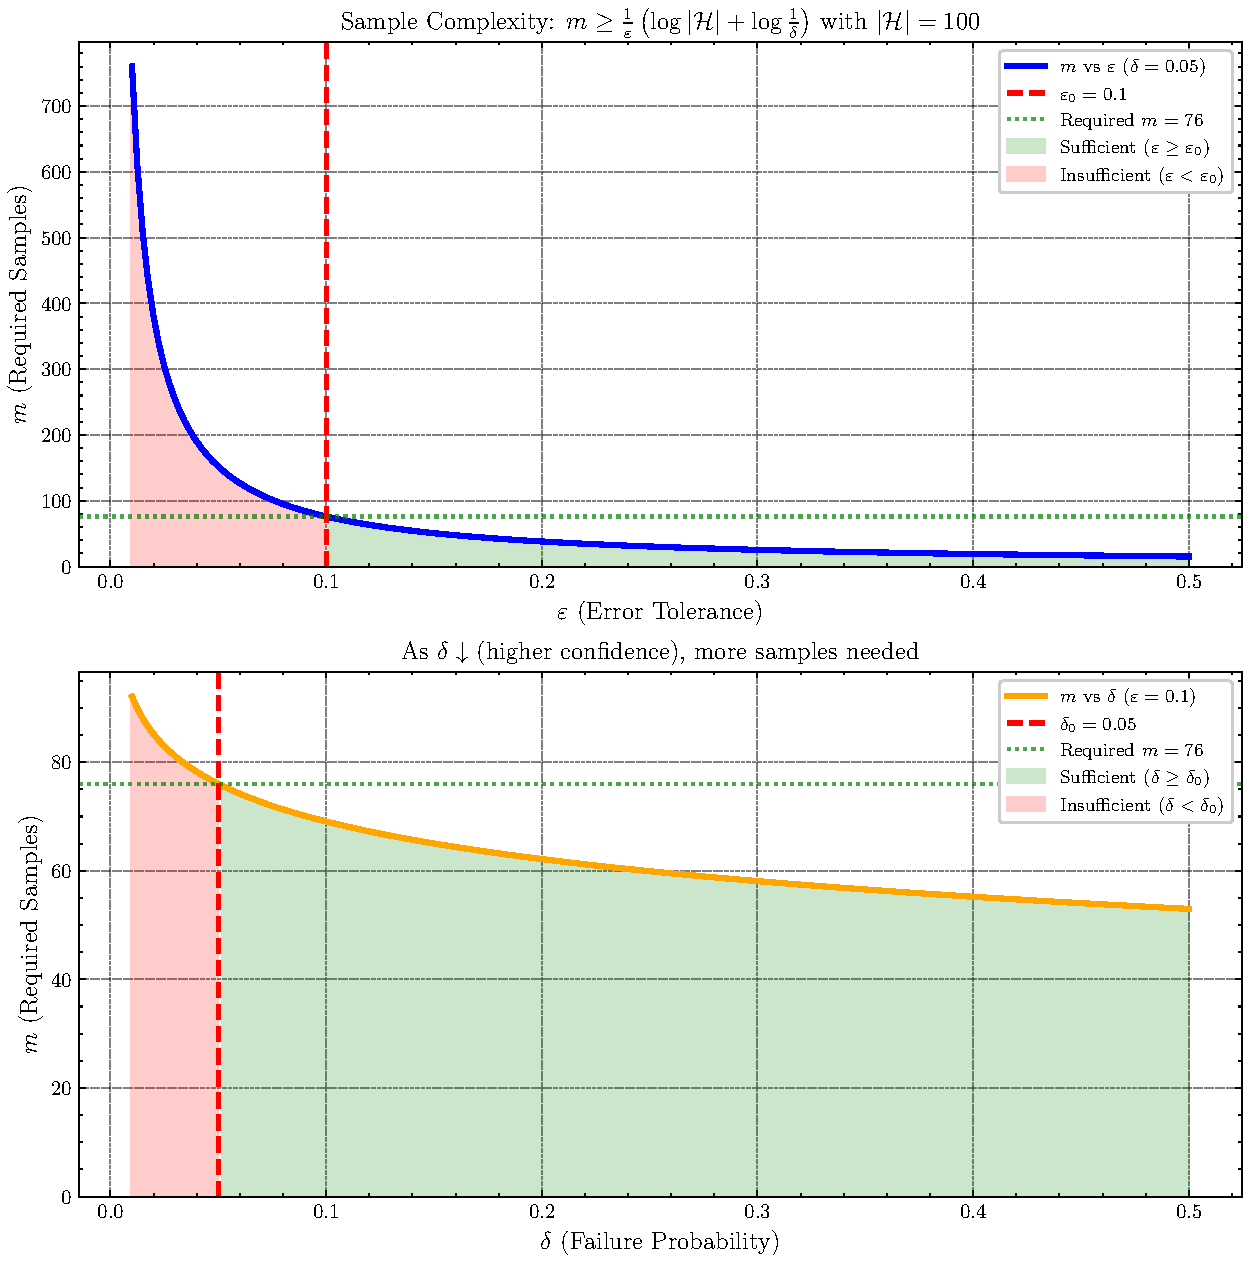
\includegraphics[width=0.7\textwidth]{pdf/PAC_sample_complexity.pdf}
    \caption{Illustration of of sample complexity in terms of cardinality $m=|\mathcal{S}|$, with respect to $\epsilon$ or $\delta$ measure.}
    \label{fig:PAC_sample_complexity}
\end{figure}

\begin{figure}[htb]
    \centering
    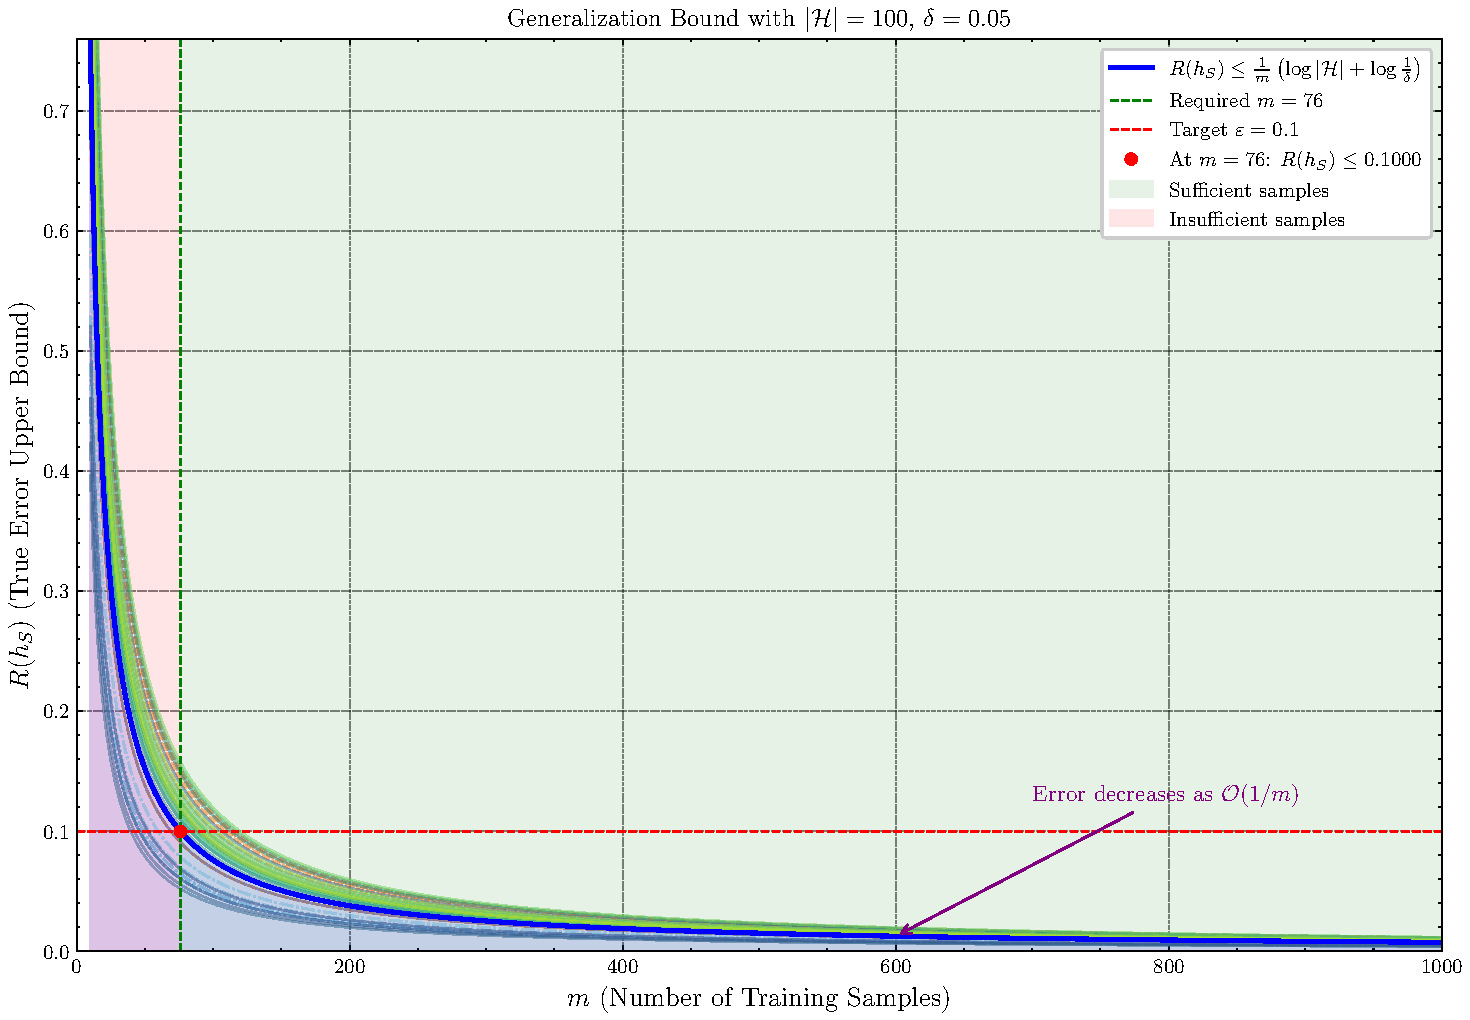
\includegraphics[width=0.7\textwidth]{pdf/PAC_generalization_bound.pdf}
    \caption{Illustration of of generalizational error/risk in terms of cardinality $m=|\mathcal{S}|$, with respect to changing $\mathcal{H}$ cardinality and $\delta$-value measure. Blurred line indicates different cases or values, the deviation is rather small, thus the bound is very tight.}
    \label{fig:PAC_generalization_bound}
\end{figure}

As for inconsistent case, the margin of error exists, thus $\mathcal{H}$ is bounded like the following. 

\begin{theorem}[Learning bound - finite $\mathcal{H}$, inconsistent case]\label{thm:theorem_inconsistent}
    Let $\mathcal{H}$ be a finite hypothesis set. Then, for any $\delta > 0$, with probability at least $1-\delta$, the following inequality holds: 
    \begin{equation}
        \forall h \in \mathcal{H}, \quad R(h) \leq \hat{R}_S (h) + \sqrt{\frac{\log{|\mathcal{H}|}+ \log{2/\delta}}{2m}}
    \end{equation}
\end{theorem}

\begin{proof}
    This proof is based on parts of \cite{10.5555/2371238} and the section about PAC theorems. In the most general case, there may be no hypothesis in $\mathcal{H}$ consistent with the labelled training sample. This, in fact is the typical case in practice, where the learning problems may be somewhat difficult or the concept classes more complex than the hypothesis set used by the learning algorithm. 

To derive the learning guarantees in the more general setting, we would use the following corollary, of which relates the generalization error and empirical error of a single hypothesis. 

\begin{col}
    Fix $\epsilon > 0$. Then, for any hypothesis $h: X \to \{0,1\}$, the following inequalities hold: 
    \begin{equation}
        \underset{S\sim \mathcal{D}^m}{\mathbb{P}} \left[\hat{R}_S (h) - R(h) \geq \epsilon\right] \leq \exp{(-2m\epsilon^2)}
    \end{equation}
    \begin{equation}
        \underset{S\sim \mathcal{D}^m}{\mathbb{P}} \left[\hat{R}_S (h) - R(h) \leq -\epsilon\right] \leq -\exp{(-2m\epsilon^2)}
    \end{equation}
    By the union bound, this implies the following two-sided inequality: 
    \begin{equation}
        \underset{S\sim \mathcal{D}^m}{\mathbb{P}} \left[|\hat{R}_S (h) - R(h)| \leq \epsilon\right] \leq 2\exp{(-2m\epsilon^2)}
    \end{equation}
\end{col}

\begin{proof}
    This can be proved using Hoeffding inequality. Recall that the inequality is stated for $Z_{1},\dots,Z_{n}$ independent random variable, for range $z_{i}\in [a_{i},b_{i}]$ with probability one, $S_{n}=\sum_{i=1}^{n}Z_{i}$ then for all $t>0$:
    \begin{equation*}
        \mathbb{P}(S_{n} - \mathbb{E}(S_n)\leq -t) \leq \exp{\left(\frac{-2t^2}{\sum (b_{i} - a_{i})^{2}}\right)}
    \end{equation*}
    and 
    \begin{equation*}
        \mathbb{P}(S_{n} - \mathbb{E}(S_n)\geq t) \leq \exp{\left(\frac{-2t^2}{\sum (b_{i} - a_{i})^{2}}\right)}
    \end{equation*}
    We can derive this for our case of the two empirical and generalization risk. Remember from \ref{thm:minimalNeu} that we have $R(h)=\mathbb{E}[\hat{R}_{S}(h)]$, we can transform the phrase to be: \begin{equation*}
        \underset{S\sim \mathcal{D}^{m}}{\mathbb{P}} \Big[ \hat{R}_{S}(h) - R(h) \geq \epsilon \Big] = \underset{S\sim \mathcal{D}^{m}}{\mathbb{P}} \Big[ \hat{R}_{S}(h) - \mathbb{E}[\hat{R}_{S}(h)] \geq \epsilon \Big]
    \end{equation*}
    with respect to $\mathcal{D}^{m}$. The form of $\hat{R}_{S}(h)$ has an additional $1/m$, hence, for simplification, we will take the form \begin{equation*}
        \underset{S\sim \mathcal{D}^{m}}{\mathbb{P}} \Big[ \hat{R}_{S}(h)/m - \mathbb{E}[\hat{R}_{S}(h)]/m \geq \epsilon m \Big]
    \end{equation*}
    By Hoeffding inequality, we have: 
    \begin{equation}
        \underset{S\sim \mathcal{D}^{m}}{\mathbb{P}} \Big[ \hat{R}_{S}(h)/m - \mathbb{E}[\hat{R}_{S}(h)]/m \geq \epsilon m \Big] \leq \exp{\left(\frac{-2m^{2}\epsilon^{2}}{\sum (b_{i} - a_{i})^{2}}\right)} 
    \end{equation}
    which is 
    \begin{equation*}
        \underset{S\sim \mathcal{D}^{m}}{\mathbb{P}} \Big[ \hat{R}_{S}(h)/m - \mathbb{E}[\hat{R}_{S}(h)]/m \geq \epsilon m \Big] \leq \exp{\left(\frac{-2m\epsilon^{2}}{(b-a)^{2}}\right)}
    \end{equation*}
    Here, our $\sum (b_{i} - a_{i})^{2}$ was replaced by a more general bound which contains only the sufficient amount of $m$ samples. This is because the sum follows from $m$ samples, which are taken as random variable of choice, then, for $a\leq Z_i \leq b$ \begin{equation*}
        \frac{m^{2}}{\sum (b_{i} - a_{i})^{2}} = \frac{m^{2}}{m(b-a)^{2}} = \frac{m}{(b-a)^{2}}
    \end{equation*}
    Since our hypothesis is mapping to $\{0,1\}$, hence our result space is discretely bounded in the normal range, the inequality reduces to 
    \begin{equation}
        \underset{S\sim \mathcal{D}^{m}}{\mathbb{P}} \Big[ \hat{R}_{S}(h)/m - \mathbb{E}[\hat{R}_{S}(h)]/m \geq \epsilon m \Big] \leq \exp{\left(-2m\epsilon^{2}\right)}
    \end{equation}
    Rearranging the left-hand-side to the original yields the inequality. Doing the same for the second case, and using the union bound, we get the two-sided inequality for $\lvert \hat{R}_{S}(h) - R(h)\rvert$. 
\end{proof}

Such bound can be naturally extended toward any arbitrary range $[a,b]$, as for Hoeffding inequality being defined on the arbitrary closed interval instead. Then, we have the general bound

\begin{equation}
    \underset{S\sim \mathcal{D}^m}{\mathbb{P}} \left[|\hat{R}_S (h) - R(h)| \leq \epsilon\right] \leq 2\exp{-\frac{2m\epsilon^2}{(b-a)^{2}}}
\end{equation}

Setting the right-hand side of the final expression to be equal to $\delta$ and solving this for $\epsilon$ yields immediately the following bound for a single hypothesis. 

\begin{col}[Generalization bound - single hypothesis]
    Fix a hypothesis $h: \mathcal{X}\to \{0,1\}$ or more generally onto $h:\mathcal{X}\to[a,b]\subset\mathbb{F}$. Then, for any $\delta > 0$, the following inequality holds with probability at least $1-\delta$: 
    \begin{equation}
        R(h) \leq \hat{R}_S(h) + \sqrt{\frac{\log{2/\delta}}{2m}}
    \end{equation}
\end{col}

The desired bound can then be realized as extending the proved corollary bound, by noticing that,  

\begin{equation}
        \hat{R}_S(h) + \sqrt{\frac{\log{2/\delta}}{2m}} < \hat{R}_S (h) + \sqrt{\frac{\log{|\mathcal{H}|}+ \log{2/\delta}}{2m}}
    \end{equation}
for all $|\mathcal{H}|$. 
\end{proof}


For a looser bound, we can ultimately use an $\epsilon$-consistent learner criteria in such case. PAC-learning setting raises some peculiar insight toward the problem itself. First, is the learning bound itself of which raises the importance of several factors --- the dataset size, $m$, of which is used as the \textbf{total resources required} for approximating such function. Furthermore, the set complexity $\mathcal{H}$ is also used, albeit questionably inconsistent in the term $\log{|\mathcal{H}|}$, which implies at least consideration on the cardinality of the hypothesis class. In a finite domain, we notice that PAC-learning of consistent case is exactly the case of interpolation, assuming non-smooth and noisy data, and the inconsistent case describe the wider range of approximation-based case, but does not consider an approximation-aware bound. The design of $|\mathcal{H}|$ also does not allow for certain exact hypothesis class size measurement, except for combinatorial case where $\mathcal{H}$ is indeed finite. Nevertheless, the bound indeed indicates that for $m$ increase, the hypothesis class often do much better in general. One particularly troublesome notion of which we will meet, in the inconsistent case, is the reversal of guarantee compared to bias-variance form. Specifically, the inconsistent, model-agnostic version of Theorem~\ref{thm:theorem_inconsistent} is as followed:
\begin{theorem}[Inconsistent case, model-agnostic, finite $\mathcal{H}$]
    For finite $\mathcal{H}$, then for any $\delta > 0$, up to $\epsilon$-accuracy, with probability at least $1-\delta$, the following inequality holds: 
    \begin{equation}
        R(h_{\mathcal{S}}) \leq \min_{h_{\mathcal{S}}\in\mathcal{H}}\hat{R}_{\mathcal{S}} (h_{\mathcal{S}}) + \sqrt{\frac{\log{|\mathcal{H}|}+ \log{2/\delta}}{2m}}
    \end{equation}
    such that 
    \begin{equation}
        \sqrt{\frac{\log{|\mathcal{H}|}+ \log{2/\delta}}{2m}} \leq \epsilon
    \end{equation}
    for $m>0$ samples. We also say that the error varies by $\mathcal{O}(\sqrt{1/m})$), such that 
    \begin{equation}
        R(h_{\mathcal{S}}) \leq \min_{h_{\mathcal{S}}\in\mathcal{H}}\hat{R}_{\mathcal{S}} (h_{\mathcal{S}}) + \mathcal{O}\left(\sqrt{\frac{\log{|\mathcal{H}|}}{m}}\right)
    \end{equation}
    We denote, again, $\hat{R}_{\mathcal{S}}$ the empirical risk given on set $\mathcal{S}$ of observations, and $h_{\mathcal{S}}$ the hypothesis obtained from dynamics regarding such observational set.  
\end{theorem}

This theorem directly indicates that, for bigger $|\mathcal{H}|$, the rate of which $m$ increases can also mitigate bias-variance, thus bigger dataset can mitigate such issues of overfitting. Indeed, we notice that $\mathcal{O}(\log{|\mathcal{H}|})\leq\mathcal{O}(m)$ linear terms, thus if the algorithm $\mathcal{A}$ exhibits such dynamics in which dataset varies, bigger hypothesis space should not increase significantly of the error measure. However, this contradicts, in a sense, with the usual term of notion to bias-variance, of which suggest otherwise, hence overfitting. Or, rather insidiously speaking, the interpretation is wrong, such that bias-variance concern fixed $m$ situation, while such bound indicates, or at least suggest, of variational $m$. 

While this does not cover the case of which $|\mathcal{H}|$ is argued to be infinite, such is then also be bounded, as for any measure, temporary called $\mu: \mathcal{H}\to \mathcal{F}$ for field $\mathcal{F}$ of which can be evaluated to $\mathbb{R}$ or else, then such is bounded in the contribution terms, and thus of the framework in which we use to express the learning dynamics. It is also then to be concerned of different classes of $\{\mu\}$ itself, as a limiting factor. This, perhaps, will lead to a potential solution of double descent. 

Indeed, a loose analogy, or rather speculation can follow. While criticisms of classical uniform-convergence PAC learning correctly observe that one-dimensional capacity sweep indeed, fail to predict or explain the modern double descent curve, such cannot be said in certain cases of the inconsistent setting. Suppose we introduce the parameter $\rho$ of the growth regime on $\mathcal{M}(\mathcal{H}):\mathcal{H}\to \mathbb{F}^{k}$ of the complexity measure or the size of the hypothesis space, in which usually $k=1$ and the value is on the real field, for $\gamma=|\mathcal{S}|$ as the sample size, such that we have $\tau$ correlates to a particular trajectory in which 
hence the escape trajectory is then controlled subsequently. We can then interpret the $\tau$ parameter as encoding the moving \textbf{interpolation threshold}. The parameter $\tau$ then can be computed, accordingly for the optimization term as 
\begin{equation}
    \mathcal{O}\left(\sqrt{\frac{\log{|\mathcal{H}|}}{m}}\right) \equiv \sqrt{\frac{\log{\tau}+ \log{2/\delta}}{2\tau}}
\end{equation}
This particular trajectory, can indeed, create certain cases where the right-half of the curve is similar to the trajectory of double descent. In general, investigation would see for 
\begin{equation}
    \mathcal{O}\left(\sqrt{\frac{\log{|\mathcal{H}|}}{m}}\right) \equiv \sqrt{\frac{\log{q(\tau)}+ \log{2/\delta}}{2q(\tau)}}
\end{equation}
for arbitrary function $q(\tau),p(\tau)$ where it should exhibit double descent terminal terms. However, this task is really hard aside from simply guessing. A simple guess on structural reformulation would be that 

\begin{align}
    &\min_{h_{\mathcal{S}\in\mathcal{H}}}\hat{R}_{\mathcal{S}}(h_{\mathcal{S}}) \approx \frac{1}{m} \left( \log{|\mathcal{H}|} + \log{\frac{1}{\delta}} \right),\\
    & \mathcal{O} \approx I \sqrt{\frac{log{(\tau - p)+\log{(2/\delta)}}}{2(\tau-p)^{\epsilon}+1}}
\end{align}
Thus the sum would be defined in a more orthodox way, as 
\begin{equation}
   \frac{1}{m} \left( \log{|\mathcal{H}|} + \log{\frac{1}{\delta}} \right) + I \sqrt{\frac{log{(\tau - p)+\log{(2/\delta)}}}{2(\tau-p)^{\epsilon}+1}}
\end{equation}
for arbitrary constant $I,p$, of which now the addition operator would be slightly adjust, such that the sum will contain only the LHS of the operator if the RHS is in its undefined domain, and otherwise they add on together. The factor $(\tau-p)$ appears in both previously the sample size $m$ and the hypothesis space size $|\mathcal{H}|$. This result is highly speculative, as it is an educated guess on the error landscape, however, still produces the approximated term on double descent. Such is then of the following hypothesis. 

\begin{hypothesis}[The flawed PAC-descent]\label{hyp:interpolation_tau}
    Let $\mathcal{H}$ be the hypothesis class, for moving parameter $\tau$ called the \textbf{interpolation threshold}. We define the interpolation offset region, $\Delta(\tau)\equiv\Delta := \tau-p$, and the regularized deviation term $\eta,\kappa>0$. Then, for specific $q(\tau)$, where we set $\tau=|\mathcal{H}|$ of the hypothesis class size, and $\tau=m$ case of the number of samples on $\mathcal{S}$, then $R(h_{\mathcal{S}})$ is bounded by, for at least probability of $1-\delta$: 
    \begin{equation}
        \begin{split}
            & R(h_{\mathcal{S}})\\
            &\leq \begin{cases}
            \frac{1}{m} \left( \log{|\mathcal{H}|} + \log{\frac{1}{\delta}} \right) & \Delta \leq -\gamma \\
            \frac{1}{m} \left( \log{|\mathcal{H}|} + \log{\frac{1}{\delta}} \right) + \lambda(\Delta) I \sqrt{\frac{log{(\tau - p)+\log{(2/\delta)}}}{2(\tau-p)^{\epsilon}+1}} & |\Delta <\gamma| \\
            \frac{1}{m} \left( \log{|\mathcal{H}|} + \log{\frac{1}{\delta}} \right) + I\sqrt{\frac{log{(\tau - p)+\log{(2/\delta)}}}{2(\tau-p)^{\epsilon}+1}} & |\Delta <\gamma| 
        \end{cases}
        \end{split}
    \end{equation}
    for $I>0$, $\lambda(\Delta)\in[0,1]$ the smooth terms on transition region, where taking $\gamma =0, \lambda(0)=1/2$ returns the discrete separation case. 
\end{hypothesis}

\begin{figure}[htb]
    \centering
    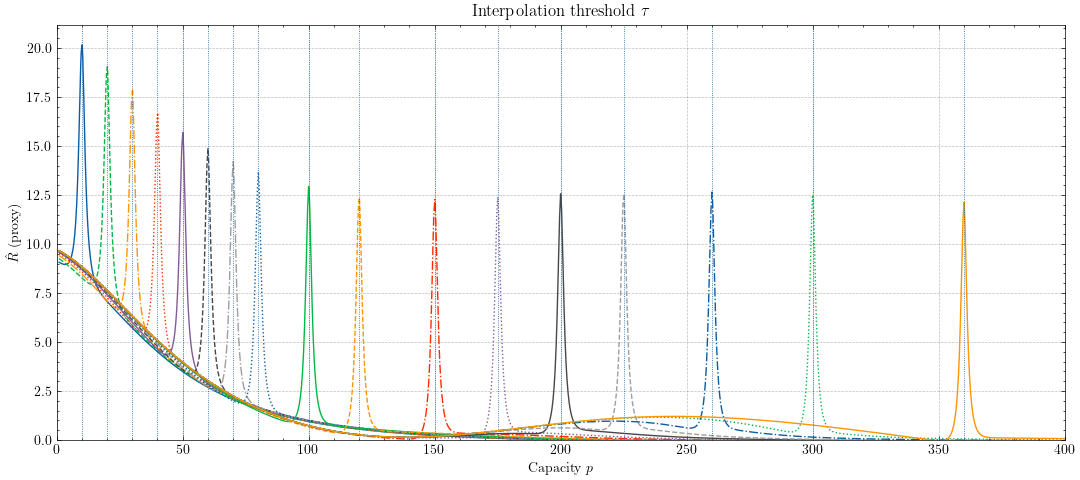
\includegraphics[width=0.9\textwidth]{media/interpolation_threshold_tau.png}
    \caption{Prediction made by certain configurations of Hypothesis~\ref{hyp:interpolation_tau}.}
\end{figure}

While imperfect, this encodes in the simplest form of PAC-system, why such bound can somewhat say of the double descent phenomena, in terms of the singular trajectory error instead. But it also reveals the problematic trouble within doing this, essentially move the theory into the untested and unprepared zone in which orthordox choices has to be made, but no interpretation is available. The ineffective side of such derivation is that: 
\begin{enumerate}[itemsep=1pt,topsep=1pt]
    \item Ill-defined terms, $\log{(\tau-p)}$ is extremely brittle and thus makes for an interpolation threshold, but theoretically, this is inexplainable, also for $(\tau-p)^{\epsilon}$ for the error $\epsilon$ bounded. Even with the regularized term, such is forced on because of necessity, not structural reason. 
    \item Circularity of the concept is that we are treating on the assumption of the escape trajectory, i.e. $(\tau-p)$, will fit both the hypothesis space size and the sample size. Indeed, such procured the double descent curve, but does not explain how and why. 
    \item Continuity and unit mismatch is indeed troublesome, as there exists no way to tell specific $q(\tau)$ that preserves the parameterization to $\tau$. Continuity means having to form piece-wise terms, hence we result in an abrupt bounding instead. 
\end{enumerate}
Inherently, $\tau$ is also empirical, and thus $q(\tau)$. Such expression in general appears in KL-convergence of PAC-Bayes, and linear models isotropic design gives $\sigma^{2}p/(m-p-1)$, which is fairly similar to what we have. Nevertheless, one should realize that current theories are not equipped to express this in particularly detailed insight. In certain cases, it only serves as heuristics or empirical presumptions, or rather theoretical speculation in a non-constructive way. Imitating double descent aside, this prompts us to seriously tackle the double descent problem, or otherwise the messiness of analysis will continue. 

\subsection{Empirical and structural algorithms}

Suppose that for a concept class $\mathcal{H}$, we can then partition it to $\mathcal{H}=\bigcup_{k\in \mathbb{N}} \mathcal{H}_{k}$ for finite $k$ hypotheses. Assume that they satisfy the uniform convergence (\cite{JMLR:v11:shalev-shwartz10a}), which means in the arbitrary path landscape, one can guarantee $\ell$-reduction, of $m$ samples on $\mathcal{S}$ to:

\begin{equation}
    \lim_{m\to \infty} \sup_{\mathcal{D}} \underset{S\sim\mathcal{D}^{m}}{\mathbb{E}} \left[ \sup_{h\in\mathcal{H}} [R(h) - R_{S}(h)] \right] = 0
\end{equation}

or, can also be expressed of equal to the following expression, for functions $\epsilon_{k}$ satisfies that for all $k$ and $\delta\in (0,1)$, $\lim_{m\to\infty}\epsilon_{k}=0$.

\begin{equation}
    \forall k \in \mathbb{N}, \quad \underset{S\sim \mathcal{D}^{m}}{\mathbb{P}} \left(\sup_{h\in \mathcal{H}_{k}} R(h) - \hat{R}_{S}(h)\leq \epsilon_{k}(m,\delta)\right) \geq 1- \delta
\end{equation}

Then such is said to be possible as a ruling dynamic when for a learning problem, the empirical risks of hypotheses in the hypothesis class converges to their population risk uniformly, with a distribution-independent rate. The result of this is that a problem then can be considered learnable with the ERM rule, for any given characterization. We state the following definition.\footnote{The reason why $r(\cdot)$ is not characterized in this preliminary section, is because of their uncertainty of effect. Hypothetically, $r(\cdot)$ is an additional structure (bias) of which apply a new gradient field in conjunction to the loss gradient field itself. This addition is uncertain of its content and analysis, since it depends on various stochastic dynamics of the model. We reserve from using regularization for now because of such reason.}

\begin{definition}
    A learning problem is learnable if there exist a learning rule $\mathcal{A}$ and a monotonically decreasing sequence $\epsilon_{cons}(m)$ such that $\epsilon_{cons}(m)\overset{m\to\infty}{\longrightarrow} 0$ and \begin{equation}
        \forall \mathcal{D} , \quad \underset{S\sim\mathcal{D}^{m}}{\mathbb{E}} \left[F(\mathcal{A}(S))-F^{*}\right] \leq \epsilon_{cons}(m),
    \end{equation}
    with $F^{*} = \inf_{h\in\mathcal{H}} R(h)$. A learning rule $\mathcal{A}$ for which this hold is denoted as a universally consistent learning rule. 
\end{definition}

There are certainly a fundamental class of rule or algorithm $\mathcal{A}$ to resolve this particular uniform convergence of classes. One of the major assumption or observation from the point of the hypothesis class, is that the hypothesis cannot know the generalization error. Thereby, one strategy is the \textit{empirical risk minimization} (ERM) method, minimizing only the empirical risk to the empirical best; then, certain measures to `generalize' this heuristically is apprehended on the hypothesis. 

\begin{definition}
    A rule $\mathcal{A}$ is an ERM (Empirical Risk Minimizer), denoted $\mathcal{A}_{ERM}$ if it minimizes the empirical risk $\hat{R}(h)=(1/m)\sum_{c\in\mathcal{C}}\ell(h,c)$, over the observational space $S$, 
    \begin{equation}
        \hat{R}_{S}(\mathcal{A}_{ERM}(S)) = \hat{R}_{S} (h_{S}) = \inf_{h\in\mathcal{H}} \hat{R}_{S}(h) 
    \end{equation}
    Hence, the ERM tries to obtain $\mathrm{ERM}(h') = \argmin_{h\in \mathcal{H}} \hat{R}(h)$. 
\end{definition}

The problem of overfitting still somewhat resides in the setting of the method. Hence, usually, we have an implicit term in addition, called the \textit{regularizer}, of which is as followed. 

\begin{definition}
    A rule $\mathcal{A}$ is an SRM (Structural Risk Minimizer), denoted $\mathcal{A}_{ERM}$ if it minimizes the empirical risk $\hat{R}(h)=(1/m)\sum_{c\in\mathcal{C}}\ell(h,c)$, over the observational space $S$, 
    \begin{equation}
        \hat{R}_{S}(\mathcal{A}_{SRM}(S)) = \hat{R}_{S} (h_{S}) + \lambda r(h)= \inf_{h\in\mathcal{H}} \hat{R}_{S}(h) + \lambda r(h)
    \end{equation}
    of the regularizing term $r(\cdot)$. Hence, the SRM tries to obtain $\mathrm{ERM}(h') = \argmin_{h\in \mathcal{H}} \hat{R}(h)$, while taking into consideration a forcing term $r$, usually defined on the model complexity. 
\end{definition}

Hence, the SRM is inherently stronger than ERM. The regularizer $\lambda r(h)$, in specific case of convex loss landscape and reasonably well-behaved irregularities between domains, and of the structural regularization term $r_{s}(h)=\sum_{i,j}w_{ij}^{2}$ for weights of $ij$ index, then we have the following theorem. 

\begin{conjecture}[ERM-SRM growth]
    Consider the regulizer $\lambda r(h)$ for $h\in\mathcal{H}$. Assuming structural regularization $r_{\mathcal{S}}(h)=\sum_{i,j}w_{ij}^{2}$ for linear-layering of $ij$ index, for ERM and SRM optimizer classes, 
    \begin{equation}
    \begin{split}
        &\mathrm{ERM}\left(\inf_{h\in\mathcal{H}} \hat{R}_{S}(h), \ell\right)\\
        &\quad \quad \quad \approx o\left(\mathrm{SRM}\left(\inf_{h\in\mathcal{H}} \hat{R}_{S}(h) + \lambda r(h), [\ell ,\lambda r(h)]\right)\right)
    \end{split}
\end{equation}
\end{conjecture}

Where the little-$o$ notation is used for saying of the optimization strength per arbitrary time-similar notion of algorithmic evolution. The reason for this change is because of the restriction domain that $\mathrm{SRM}$ indicted on the model optimization landscape. Effectively, we introduce the structural bias $\lambda r(h)$ that forces the morph of the total loss landscape. In well-behaved case, this is usually effective to a point, however in realistic system and pathological cases, such can lead to the $c'$ approximation in $c$-space, just as we introduced in the reformulation of learning system. In this paper, we would like to presume the ERM method in question as the famous \textit{gradient descent}. We refer to \cite{achlioptas_stochastic_nodate,ruder_overview_2017} for general view of the algorithm, and \cite{zhang_gradient_2019} for a source on particularly gradient descent algorithm on deep learning models. 

One particularly troublesome and should take serious consideration into interpreting it, is the fact of the insufficiency on ERM. The following proposition is rather questionable. 
\begin{proposition}
    For any sample $S$, the following inequality holds for the hypothesis returned by ERM: 
    \begin{equation}
        \mathbb{P}\Big[R(h_{S}')- \inf_{h\in \mathcal{H}}R(h) > \epsilon\Big] \leq \mathbb{P}\Big[ \sup_{h\in \mathcal{H}} \lvert R(h)- \hat{R}_{S}(h) \rvert > \frac{\epsilon}{2} \Big]
    \end{equation}
\end{proposition}
We will prove this proposition in later section. For now, this proposition bounds the error of ERM, with respect to the probability of the generalization distance $\lvert R(h)- \hat{R}_{S}(h)\rvert$ between the two errors. As we might have suspected, the performance of ERM is typically very poor. This is because the algorithm disregards the complexity of the hypothesis set $\mathcal{H}$: in practice, either it is not complex enough, in which case the error can be large, or $\mathcal{H}$ is so rich, that the complexity makes the model shoot out of the complexity range. Additionally, in many cases, determining the ERM solution is computationally intractable. 

\subsection{The PAC-ERM notion}

Without restricting ourselves to specific ERM construction, we can still apply PAC on the set of ERM algorithms in its generality of itself. Within such understanding, the empirical risk minimization strategy is often motivated by the hope that \textit{$R$(h) and $\hat{R}(h)$ are not too far-distant apart}. Particularly, it also implicitly agree with statements conjectured with law of large number, for $n\to\infty$, $|R(h)-\hat{R}(h)|\approx \epsilon$ of irreducible noise. To what extent is this true, we have to take certain boundary on which might have been previously shown. We refer to authoritative introductory texts like \cite{Alquier_2024}, for both PAC-ERM and later sections on PAC-Bayes variation. 

\begin{proposition}[\cite{Alquier_2024}]\label{prop:PAC_ERM_1}
    For any $h\in\mathcal{H}$, for any $\delta\in(0,1)$, 
    \begin{equation}
        \mathbb{P}_{S}\left( R(h) > \hat{R}(h)+ C\sqrt{\frac{\log{(1/\delta)}}{2n}}\right)\leq \delta
    \end{equation}
\end{proposition}
\begin{proof}
    Applying Hoeffding's inequality onto $U=\mathbb{E}[\ell_{i}(h)]-\ell_{i}(h)$, 
    \begin{equation}
        \mathbb{E}_{S}\left[\exp{tn[R(h)-\hat{R}(h)]}\right] \leq \exp{[(nt^2C^2)/8]}
    \end{equation}
    For any $s>0$, we have by Markov's inequality, 
    \begin{equation}
        \begin{split}
            \mathbb{P}_{S}(R(h)-\hat{R}(h)>s) 
            & = \mathbb{P}_{S} \left(\exp{nt[R(h)-R]}> \exp{(nts)}\right)\\
            & \leq \frac{1}{\exp{(nts)}} \mathbb{E}_{S}\left[e^{nt[R(h)-\hat{R}(h)]}\right]\\
            & \leq \exp{\left(\frac{nt^2C^2}{8}-nts\right)}
            \end{split}
    \end{equation}
    We can make this bound as tight as possible, by optimizing the choice of $t$. For $t=4s/C^{2}$, we have 
    \begin{equation}
        \mathbb{P}(R(h)-\hat{R}(h)>s) \leq \exp{\left(\frac{-2ns^2}{C^2}\right)}
    \end{equation}
    This means that, for a given $h$, the empirical risk $\hat{R}(h)$ cannot be much smaller than the risk $R(h)$. The order of this "much smaller" can be better understood by introducing $\delta=\exp{(-2ns^2/C^2)}$, of which substituting $\delta$ to $s$ yields the required proposition. 
\end{proof}

Proposition~\ref{prop:PAC_ERM_1} bounds the asymptotic term such that $R(h)$ will exceed $\hat{R}(h)$ by certain margin, at worst $1/\sqrt{n}$. However, this is not enough to justify the use of ERM (which indeed use the near-space approximation from empirical to general risk), since the proof only applies for $h$ that was fixed above in terms of complexity. For those that is implicit of the data itself, we cannot apply them\footnote{This means models such ass \textit{support vector machine} (SVM) or \textit{Gaussian process regression} of which the empirical optimization function and the hypothesis itself, relies on the number of data points available.}. The usual approach though, is to use the inequality 
\begin{equation}
    R(h_{ERM}) - \hat{R}(h_{ERM}) \leq \sup_{h\in\mathcal{H}} \left[R(h)-\hat{R}(h)\right]
\end{equation}
and to prove a version of Proposition~\ref{prop:PAC_ERM_1} that would hold uniformly on $\mathcal{H}$. 
\begin{theorem}
    Assume that $\mathrm{card}(\mathcal{H})=M<+\infty$, for any $\delta\in(0,1)$, 
    \begin{equation}
        \mathbb{P}_{S}\left( R(h_{ERM}) \leq \inf_{h\in\mathcal{H}} \hat{R}(h) + C\sqrt{\frac{\log{(M/\delta)}}{2n}} \right) \geq 1 - \delta
    \end{equation}
\end{theorem}
\begin{proof}
    We upper bound the supremum in the inequality by 
    \begin{equation}
        \begin{split}
            \sP_{S} \left(\sup_{h\in\mathcal{H}}[R(h)-\hat{R}(h)>s]\right)
            & = \sP_{S} \left(\bigcup_{h\in\mathcal{H}} \left\{ [R(h)-\hat{R}(h)]>s \right\} \right)\\
            & \leq \sum_{h\in\mathcal{H}} \mathbb{P}_{S}(R(h)-\hat{R}(h)>s)\\
            & \leq M\exp{\left(\frac{-2ns^2}{C^2}\right)}
        \end{split}
    \end{equation}
    This time, put $\delta = M\exp{(-2ns^2/C^2)}$ we gain 
\begin{equation}
     \mathbb{P}_{S}\left( \sup_{h\in\mathcal{H}}[R(h)-\hat{R}(h)] \leq  C\sqrt{\frac{\log{(M/\delta)}}{2n}} \right) \leq \delta
\end{equation}
Thus it satisfies 
\begin{equation}
     \mathbb{P}_{S}\left( \sup_{h\in\mathcal{H}}[R(h)-\hat{R}(h)] \leq  C\sqrt{\frac{\log{(M/\delta)}}{2n}} \right) \geq 1-\delta
\end{equation}
Using the inequality
\begin{equation}
    \mathbb{P}_{S}\left( R(h_{ERM}) \leq \hat{R}(h_{ERM})  C\sqrt{\frac{\log{(M/\delta)}}{2n}} \right) \geq 1-\delta    
\end{equation}
As $\mathcal{H}$ is finite, $\hat{R}(h_{ERM})=\inf_{h\in\mathcal{H}}\hat{R}(h)$.
\end{proof}
This bound coincides for the \textit{Probably Approximately Correct} PAC-bounds, specifically for algorithm of ERM principle, since it approximates $R(h_{ERM})$ within $C\sqrt{\log{(M/\delta)}/2n}$ with probability $1-\delta$, and once again, under very strong arguments. Certain version of this theorem's result can be derived to `predict' double descent, but not giving its the diagnostic view. 
\subsection{Noise, \cite{10.5555/2371238}}

Using the notion of the Bayes classifier and Bayes error, one can define the \textit{noise} \index{noise} of a given learning setting under PAC-learning consideration, as followed. 
\begin{definition}[Noise]
    Given a distribution $\mathcal{D}$ over $\mathcal{X}\times \mathcal{Y}$, the \textit{noise} at point $x\in \mathcal{X}$ is defined by \begin{equation*}
        noise(x) = \min_{x\in \mathcal{X}} \{\mathbb{P}[1\mid x], \mathbb{P}[0\mid x]\}
    \end{equation*}
    The average noise or the noise associated to $\mathcal{D}$ is then the minimum possible error aside from intrinsic model error, and is calculated by $\mathbb{E}[noise(x)]$
\end{definition}
Thus, the average noise is precisely the Bayes error, that is, $noise = \mathbb{E}[noise(x)]=R^{*}$. The noise is a characteristic of the learning task indicative of its level of difficulty. A point $x\in \mathcal{X}$, for which noise is close to $1/2$, is sometimes referred to as \textit{noisy} and is of course a challenge for accurate prediction. Such is understandable, and is often enough, however, we note that structurally, it is missing particular components or decomposition components that would eventually make up the builks of its claims. 

\section{The bias-variance - double descent dilemma}

Before continuing further, we must review the problem statement that led to the problem of double descent. We will have a look at the theory, the original conflict, and the illustrative phenomenon in action. In general, the learning setting in consideration of statistical learning theory is often supervised learning, for guarantee of a plausible upper bound result. 

\subsection{Bias-variance tradeoff}

In classical sources, \cite{James2021,goodfellow2016deep,STL_Hajek_Maxim_2021,10.5555/2371238,10.5555/2621980}, the principle of bias-variance tradeoff is a classical principle used in the categorization of technique called \textit{model selection}. Specifically, this refers to the progress of choosing the best predictor $h^{*}$ that minimize the generalization error that is the main goal of a particular machine learning model, during the process of training and inference. Originally, the theory that bias and variance often come in to conjunction is \textbf{Estimation theory}, of which there exists an estimator $\hat{\theta}$ that use a set of observations, to estimate the concept, or the underlying mechanics of certain system that outputted the observation set, by the \textbf{probabilistic perspective} - that is, it is governed by appearance by an independently and identically distributed process of parameterized probability $\theta\in \Theta$. Here, parameterized means being expressed by a set, often finite, of parameters, by \cite{LehmannCasella_theory_1998,liam_statistics_2005}. It is only when \cite{6797087} introduced it to machine learning that we have an equivalent structure that is similar to bias-variance in machine learning. 

\subsubsection{Precursor (\cite{6797087})}

The original definition of bias-variance tradeoff by \cite{6797087} is first constructed using the means-square error, which is regarded as a normal measure in the real encoding space. Their approach is to justify bias-variance via decomposition of the loss function $\ell$, for such to find an alternative reasonable form of such loss landscape. Suppose of a regression problem to construct a hypothesis function $f(x)$ from $(x_{1},y_{1},\dots,x_{N},y_{N})$ for the purpose of generalization - that is, predicting unseen variational values for different pair $(x_{j}, \mathord{?})$ such that $\mathord{?}=y_{j}+\epsilon$ for a conceivable implicit error. To be explicit about the relation of this problem, or $f$ on the given data $\mathcal{D}=\{(x_i, y_i)\mid i \leq N\}$, denote $f(x;\mathcal{D})$ instead of $f$, the natural mean-square measure as a predictor is: 
\begin{equation}
    \mathcal{M}(f,y) = \mathbb{E} \left[((y-f(x;\mathcal{D})))^{2}\mid x, \mathcal{D}\right] 
\end{equation} for $\mathbb{E}[\cdot]$ the expectation wrt to a distribution $P$. Decomposing the right-hand side, we have: 
\begin{equation}
    \begin{split}
        \mathcal{M}(f,y) &= \mathbb{E} \left[((y-f(x;\mathcal{D})))^{2}\mid x, \mathcal{D}\right] \\
        &= \mathbb{E}\left[(y-\mathbb{E}[y\mid x])^{2}\mid x,\mathcal{D}\right] + (f(x;\mathcal{D})-\mathbb{E}[y\mid x])^{2}
    \end{split}
\end{equation}
Here, $\mathbb{E}\left[(y-\mathbb{E}[y\mid x])^{2}\mid x,\mathcal{D}\right]$ does not depend on $\mathcal{D}$, but simply the statistical variance of $y$ given $x$. The term $(f(x;\mathcal{D})-\mathbb{E}[y\mid x])^{2}$ is considered a natural measure of effectiveness on $\mathbb{R}^{n}$ as a singular predictor of $y$. Now, for $\mathbb{E}_{\mathcal{D}}\left[(f(x;\mathcal{D})-\mathbb{E}[y\mid x])^{2}\right]$ which depends on the training set $\mathcal{D}$ in its computation, is decomposed into the form of \textit{bias-variance decomposition} terms, by derivation: 
\begin{equation}
    \begin{split}
        &\mathbb{E}_{\mathcal{D}} \left[(f(x;\mathcal{D})-\mathbb{E}[y\mid x])^{2}\right] \\
        &\quad \quad = \underbrace{\left\{ \mathbb{E}_{\mathcal{D}}[f(x;\mathcal{D})] - \mathbb{E}[y\mid x] \right\}^{2}}_{\text{bias term}} \\
        &\quad\quad + \underbrace{\mathbb{E}_{\mathcal{D}} \left\{(f(x;\mathcal{D})- \mathbb{E}_{\mathcal{D}}[f(x;\mathcal{D})])^{2}\right\}}_{\text{variance term}}
    \end{split}
\end{equation}

We summarize this in the following statement. 

\begin{theorem}[Bias-variance decomposition]
    Suppose the model $f(x;\mathcal{D})$ for the data $\mathcal{D}=(x_i, y_i)$ and its parameter $x$ is defined. For $y_{i}$ of the target concept's responses $y$, and consider a regression problem with the loss measure $\mathcal{M}(f,y)$ of mean squared risk, the following statement is true: \begin{equation}
        \begin{split}
            \mathbb{E}\big[\mathcal{M}(f,y)\big] &= \mathcal{B}(f,y) + \mathcal{V}(f,y) \\
            &+ \mathbb{E}\Big[\mathbb{E} \left[((y-f(x;\mathcal{D})))^{2}\mid x, \mathcal{D}\right]\Big]
        \end{split}
    \end{equation}
    for $\mathbb{E}[\:\cdot\mid x, \mathcal{D}]$ any expression with dependencies on $x$ and $\mathcal{D}$. The bias and variance term is subsequently expressed by 
    \begin{align}
        \mathcal{B}(f,y) &= \underbrace{\left\{ \mathbb{E}_{\mathcal{D}}[f(x;\mathcal{D})] - \mathbb{E}[y\mid x] \right\}^{2}}_{\text{bias }}, \\
        \mathcal{V}(f,y) &=\underbrace{\mathbb{E}_{\mathcal{D}} \left\{(f(x;\mathcal{D})- \mathbb{E}_{\mathcal{D}}[f(x;\mathcal{D})])^{2}\right\}}_{\text{variance}}
    \end{align}
\end{theorem}

\sidecaptionvpos{figure}{c}
\begin{SCfigure}[1.3][htb]
  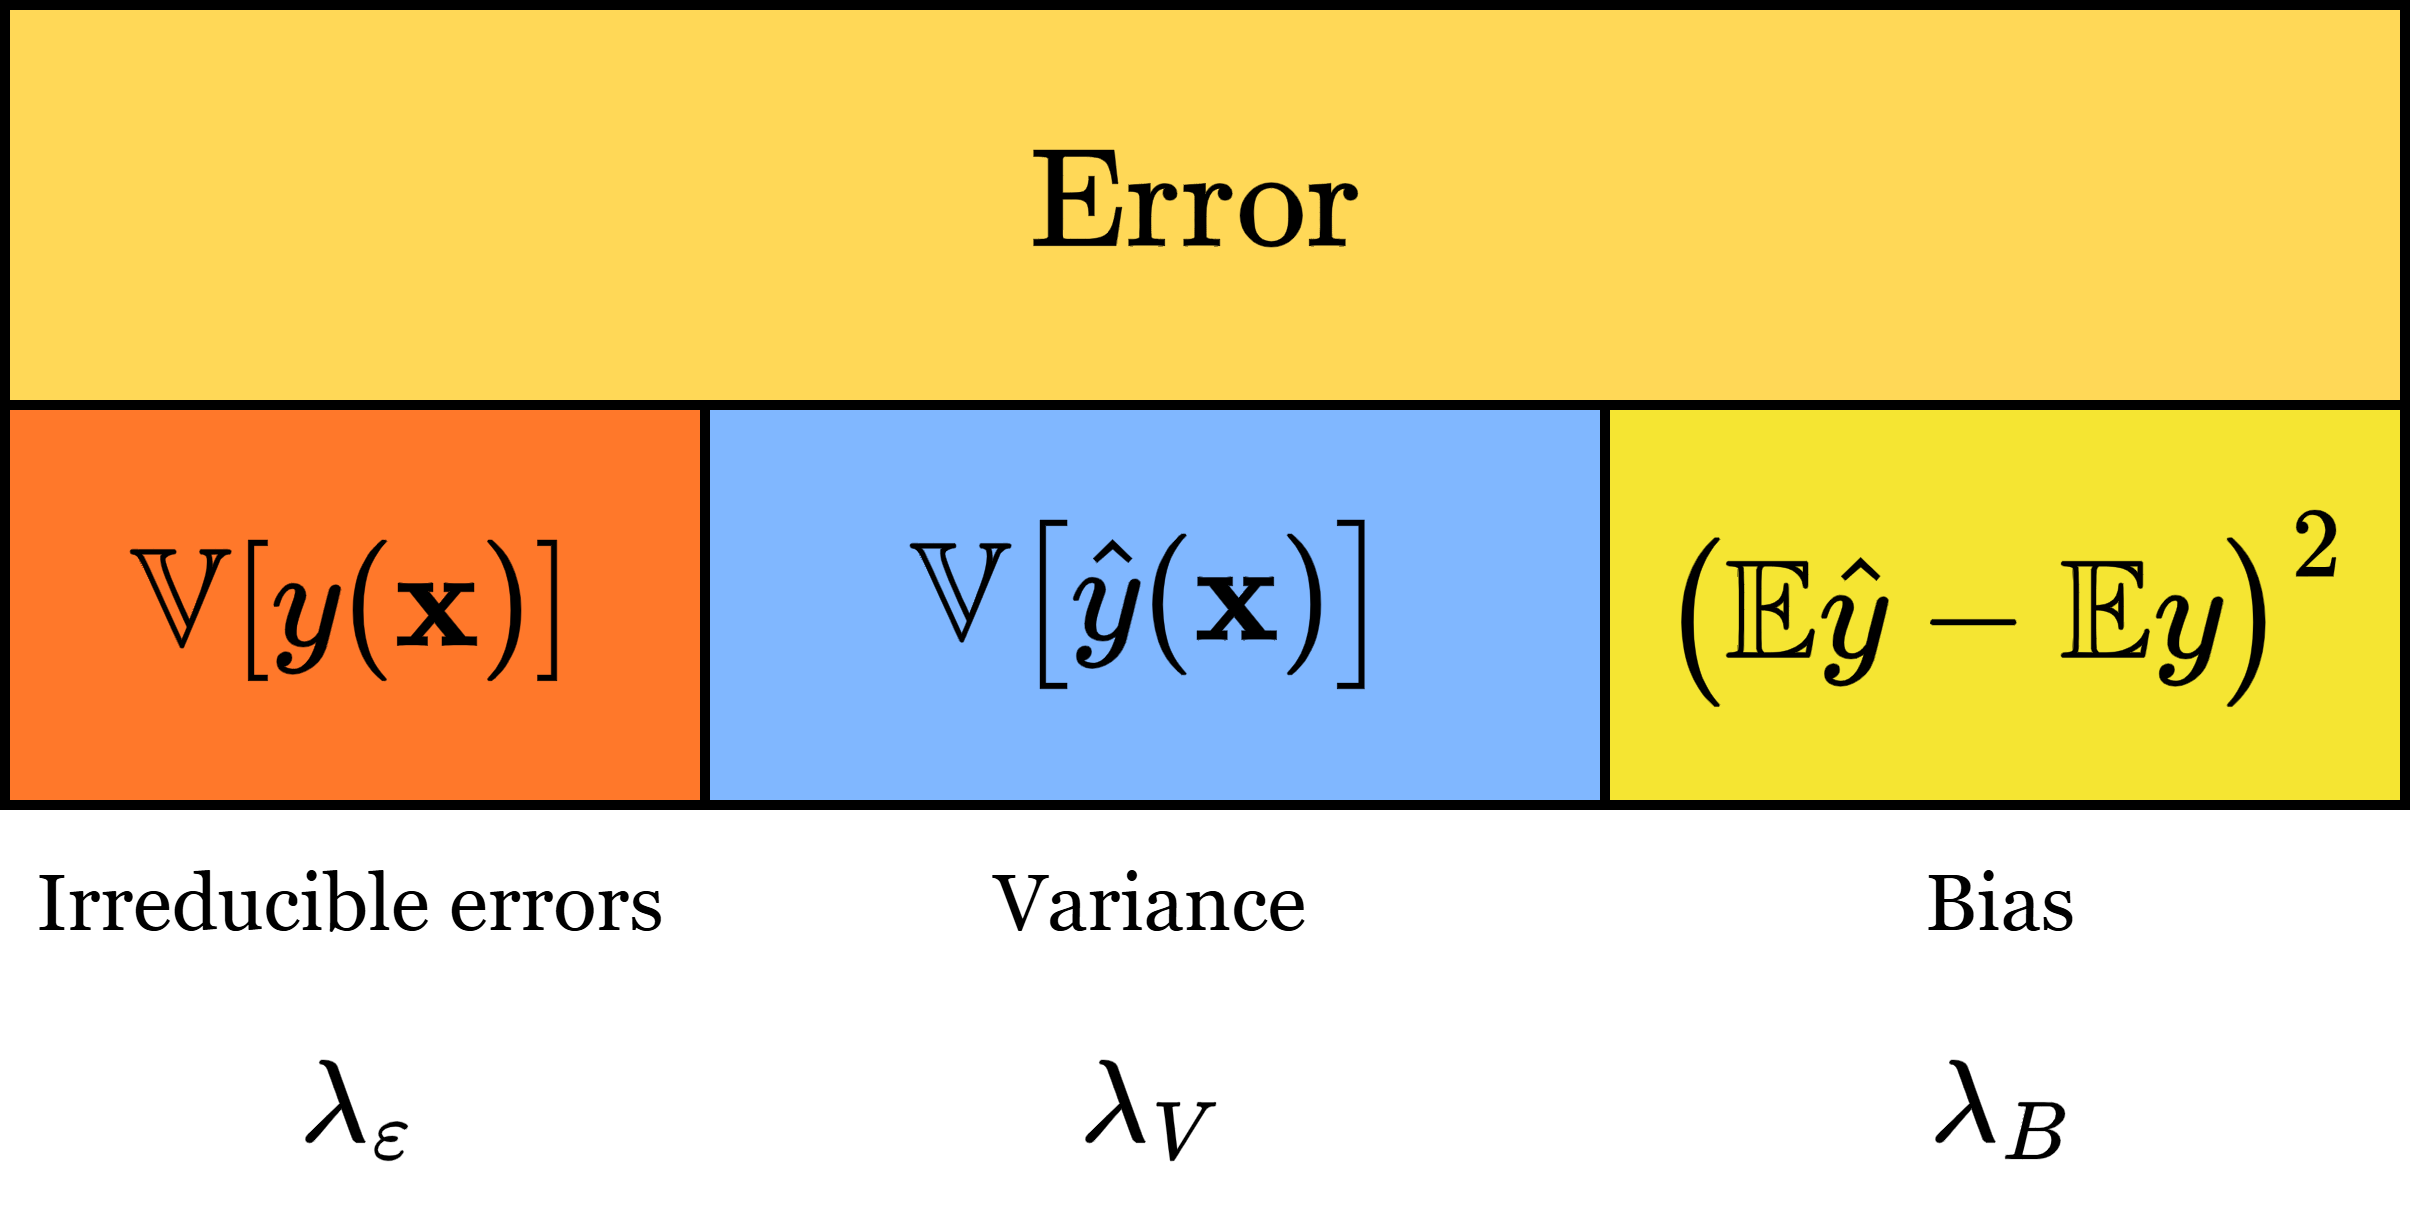
\includegraphics[width=0.4\textwidth]{media/error_decomposition.png}
  \caption{\textbf{Decomposition of the error term into 3 parts}. Respectively, the irreducible error $\mathbb{V}[y(\mathbf{x})]$, the variance (blue) and the bias (dark yellow). All of them are assumed to take up 100\% of the error observed in such composition. The proportion is included using the three coefficient $\lambda_{\epsilon},\lambda_{V},\lambda_{B}$ where $\lambda_{\epsilon}+\lambda_{V}+\lambda_{B}=1$.}
\end{SCfigure}

The above decomposition principle is often expressed into a form where there exists the intrinsic noise \cite{brown2024biasvariance}: 
\begin{equation}
    \begin{split}
        \mathbb{E}_D \left[ \mathbb{E}_{xy} \left( y - \hat{f}(x) \right)^2 \right]
        &= 
         \mathbb{E}_x \left[ \left( y^* - \mathbb{E}_D[\hat{f}(x)] \right)^2 \right]\\
        &+ \mathbb{E}_x \left[ \mathbb{E}_D \left( \hat{f}(x) - \mathbb{E}_D[\hat{f}(x)] \right)^2 \right] \\
        &+ \mathbb{E}_{xy} \left[ \left( y - y^* \right)^2 \right]
    \end{split}
    \end{equation}
In all, almost all representation of bias-variance decomposition are the same. For simplicity of notation, we adopt the similar form in the standard case of the paper \cite{adlam2020understandingdoubledescentrequires}: 
\begin{equation}
    \E \qa{\hat{y}(\bfx)-y(\bfx)}^2 = \pa{\E\hat{y}(\bfx) - \E y(\bfx)}^2 + \V\qa{\hat{y}(\bfx)} + \V\q{y(\bfx)}
\end{equation}
A main common theme of criticism toward bias-variance tradeoff is the fact that the decomposition is much more general, and intrinsic for the class of \textit{mean squared loss}. However, when considering the naturalness of an error measure and then its direct applicant, mean square error on real space of sufficient support and measure comes of as a very natural choice of an error measure, at least in consideration of the regression setting; for that, we then can also define classification as another top-layer above a regression's similar real continuous space, i.e. a decision layer. Furthermore, it can also be shown \cite{brown2024biasvariance,PfauBregmanDivergence} that it also holds for the class of Bregman divergence measure. 

What does the decomposition say about model selection principle in general? In general, bias-variance is typically presented of its decomposition only, and the asymptotic prediction of its behaviours. In fact, one of the reason that it became the rule-of-thumb for ML practitioner, as well as generally statistical learning (\cite{lafon_understanding_2024} provides a quite rigorous treatment of bias-variance tradeoff in the section on statistical learning theory) solidify the trade-off as a particular model selection principle. Generally, this tradeoff can be summarized as followed: 
\begin{theorem}[Bias-variance tradeoff]\label{thm:bias-variance}
    For the expected loss of any given hypothesis $h$, the bias $\mathcal{B}(f,y)$ and variance $\mathcal{V}(f,y)$ is inversely proportional, that is, $\mathcal{B}(f,y)\propto \lambda^{-1} \mathcal{V}(f,y)$ for some proportionality $\lambda$ that may or may not be constant. In the most general case possible, $\lambda = -1$ on the entire error range. 
\end{theorem}

The tradeoff is then of inverse proportionality. Indeed, statistically, we have such tradeoff on a statistical framework in a more concrete sense. For the bias to increase, variance will increase, of which the criterion is inverse - we would like to have more bias but lower variance, and vice versa, according to such theory.

\subsubsection{Expansion and variations}

The bias-variance decomposition and tradeoff is not general. Indeed, works, by \cite{6797087,sharma_bias-variance_2014,domingos_unifeid_2000,adlam2020understandingdoubledescentrequires,yang_rethinking_2020} and more all attempted to reconstruct and reformulate bias-variance, and it did leave out a picture of uncertainty regarding the concept. Specifically, there are certainly different way to do the bias-variance decomposition, as classified in \cite{adlam2020understandingdoubledescentrequires} paper. Some of this are particularly specialized in \textit{neural network} training, basing on the main structure of modern machine learning in neural network formalism. 
\begin{enumerate}
    \item \textbf{Semiclassical approach}: The semiclassical approach is fairly simple. We can rewrite to another variation of the classical approach to be \begin{equation}
        \begin{split}
            \underset{h\in\mathcal{H}}{\mathbb{E}[\ell(h)]} &= \mathbb{E}_{x}\mathbb{E}_{\epsilon}\left[\hat{y}(x)-y(x)\right]^{2}\\
             &= \mathbb{E}_{x}\left(\mathbb{E}_{\epsilon}[\hat{y}(x)]-y(x)\right)^{2} + \mathbb{E}_{x}\mathbb{V}_{\epsilon}\left[\hat{y}(x)\right]  
        \end{split}
    \end{equation}
    and instead, consider the \textit{structural conformation} of the decomposition, or rather, taking the expectation within $\theta\in \Theta$ of the structural description of $h\in\mathcal{H}$. Then, we shall have 
    \begin{equation}
        \begin{split}
            \underset{h\in\mathcal{H}}{\mathbb{E}_{\mathrm{SC}}[\ell(h)]} 
            &= \mathbb{E}_{x}\mathbb{E}_{\theta}\mathbb{E}_{\epsilon}\left[\hat{y}(x)-y(x)\right]^{2} \\
            &= \mathbb{E}_{x}\mathbb{E}_{\theta}\left(\mathbb{E}_{\epsilon}[\hat{y}(x)]-y(x)\right)^{2} + \mathbb{E}_{x}\mathbb{E}_{\theta}\mathbb{V}_{\epsilon}\left[\hat{y}(x)\right]
        \end{split}
    \end{equation}
    Do note that the order matters, since the expectation can be constant of a given ordering. And expected value over constant is just the constant. 
    \item \textbf{Symmetric decomposition}: This approach is fairly difficult, we refer to the paper itself of its own justification on the decomposition. The symmetric decomposition relies on the shape of the input, $\mathcal{X}=\{P,D,\epsilon\}$, of which you can remove the $\epsilon$ term and retain some decomposition on $P$ and $D$ per distribution. 
\end{enumerate}

\subsubsection{Generalized decomposition}

According to \cite{domingos_unified_aaai_2000,domingos_unified_2000}, the bias-variance decomposition can usually be treated as being controlled by three factor error, with their respective coefficients $\lambda=(\lambda_{1},\lambda_{2},\lambda_{3})$ for such: 
    \noindent 
    \begin{equation*}
        \begin{split}
            &\mathbb{E}_{\mathcal{D}} \left[d((f,\mathbb{E}[y\mid x])\right] \\
            & \quad = \lambda_{1} \mathrm{Bias}(f,y) + \lambda_{2}\mathrm{Var}(f,y)+ \lambda_{3}\epsilon(\mathcal{D})\\ 
            & \quad = \lambda_{1}\underbrace{\left\{ \mathbb{E}_{\mathcal{D}}[f(x;\mathcal{D})] , \mathbb{E}[y\mid x] \right\}}_{\text{bias term}} \\
            &\quad\quad +\lambda_{2} \underbrace{\mathbb{E}_{\mathcal{D}} \left\{(f(x;\mathcal{D}), \mathbb{E}_{\mathcal{D}}[f(x;\mathcal{D})])\right\}}_{\text{variance term}} \\
            &\quad\quad +\underbrace{\lambda_{3}\epsilon}_{\text{irreducible error}}
        \end{split}
        \end{equation*}
where $\epsilon(\mathcal{D})$ is the irreducible error of the system, depends (theoretically) on the intrinsic imperfection of the dataset $\mathcal{D}$. This method of which the bias-variance-irreducible error are `fit' into the total error by three coefficients $\lambda_{1},\lambda_{2},\lambda_{3}$ instead. This does not only scale up the B-V-IE triplet, but also leaves out the inexplainable gap between the scaling, and the actual normal measure. 

\subsubsection{Bias-variance algorithm}

\subsubsection{Functional approximation algorithm}

Usually, the optimization problem is evaluated empirically of its bias-variance metric. That is, we test singular models successively, and then choose the generally best --- usually within bias-variance tradeoff. This can be expressed as a function for theorem \ref{thm:bias-variance}. 

\subsubsection{Approximation-estimation tradeoff}

Another closely related notion to bias-variance is the concept of approximation-estimation tradeoff. We refer to \cite{10.5555/2371238,lafon_understanding_2024} for some analysis and mentions. 

Let $\mathcal{H}$ be a family of functions mapping $\mathcal{X}\to\{1,-1\}$. This is the particular case of \textbf{binary classification}, in which can be straightforwardly extended to different tasks and loss functions. The \textit{excess error} of a hypothesis $h\in\mathcal{H}$, is the difference between its error $R(h)$ and the Bayes error $R^{*}$. This can be decomposed to be the following: 

\begin{equation}
    R(h) - R^{*} = \Big( R(h) - \inf_{h\in \mathcal{H}} R(h) \Big) + \Big( \inf_{h\in \mathcal{H}} R(h) - R^{*} \Big)
\end{equation}

The first bracket contains the \textbf{estimation error}, and the second bracket contains what is called the \textbf{approximation error}. The estimation error depends on the hypothesis $h$ selected. It measures the error of $h$ with respect to the infimum of the error achieved by hypotheses in $\mathcal{H}$, or that of the best-in-class hypothesis $h^{*}$ when that infimum is reached. The approximation error measures how well the Bayes error can be approximated using $\mathcal{H}$. It is a property of the hypothesis set $\mathcal{H}$, a measure of its richness. 

Model selection consists of choosing $\mathcal{H}$ with a favourable trade-off between the approximation and the estimation error. However, in the most general case, this will be done, but not in practice, as it requires the underlying distribution $\mathcal{D}$ to be known to determine $R^{*}$, which is not possible. In contrast, the estimation error can be bounded, or can be analysed, using particular metric and analysis. It is however, worth to note that bias-variance and approximation-estimation have a very complicated relationship, for example, in \cite{brown2024biasvariance} shown that they are indeed not the same, and is in fact two different decomposition, where one is the others' component. To see this, let us compare the two of them in details. 

\subsection{Double descent}

Nevertheless, of bias-variance and the analogous statistical learning theory concept, the target is the same. It is the dilemma of which is presented in \textbf{Occam's razor}, for choosing the sufficient model of good complexity, or bias, for tradeoff of its generalization ability, or variance. Then there must exist a sweet spot between the axis of bias and variance, since they are as exhibited above inversely proportional to each other. However, double descent seemingly broke the status quo, and insists on an interesting phenomenon - under the same setting, if we `crank' the complexity high enough, we will then reach a point then called the \textbf{interpolation threshold}, such that the trend reverse and the error rate, instead of being theorized to go up, goes down to a certain line of lower bound. 

The first identification of the double descent phenomena dated back to the paper of Belkin - \cite{belkin_reconciling_2019}, in which the title is literally "reconciling" modern machine learning practice and the bias-variance tradeoff. In modern machine learning practice, or state-of-the-art developments, models are now bigger than ever. If to notice, we will see that currently models are inherently large, for example, a normal large language model will have from 900 millions (900M) to a few billions, for example 10 billions (10B) parameters. That is not taking into account the overall dynamics and structure of the model, which dictates the operating range and efficiency of the model itself. These model, based on the neural network architecture are somewhat trained to exactly fit (or interpolate) the data, almost certainly so that it turn from a prediction setting to an estimation setting. By statistical learning theory, this would be considered overfitting, and yet, they often obtain very high accuracy on test data.

\begin{figure*}
    \centering
    \begin{tabular}{cc}
    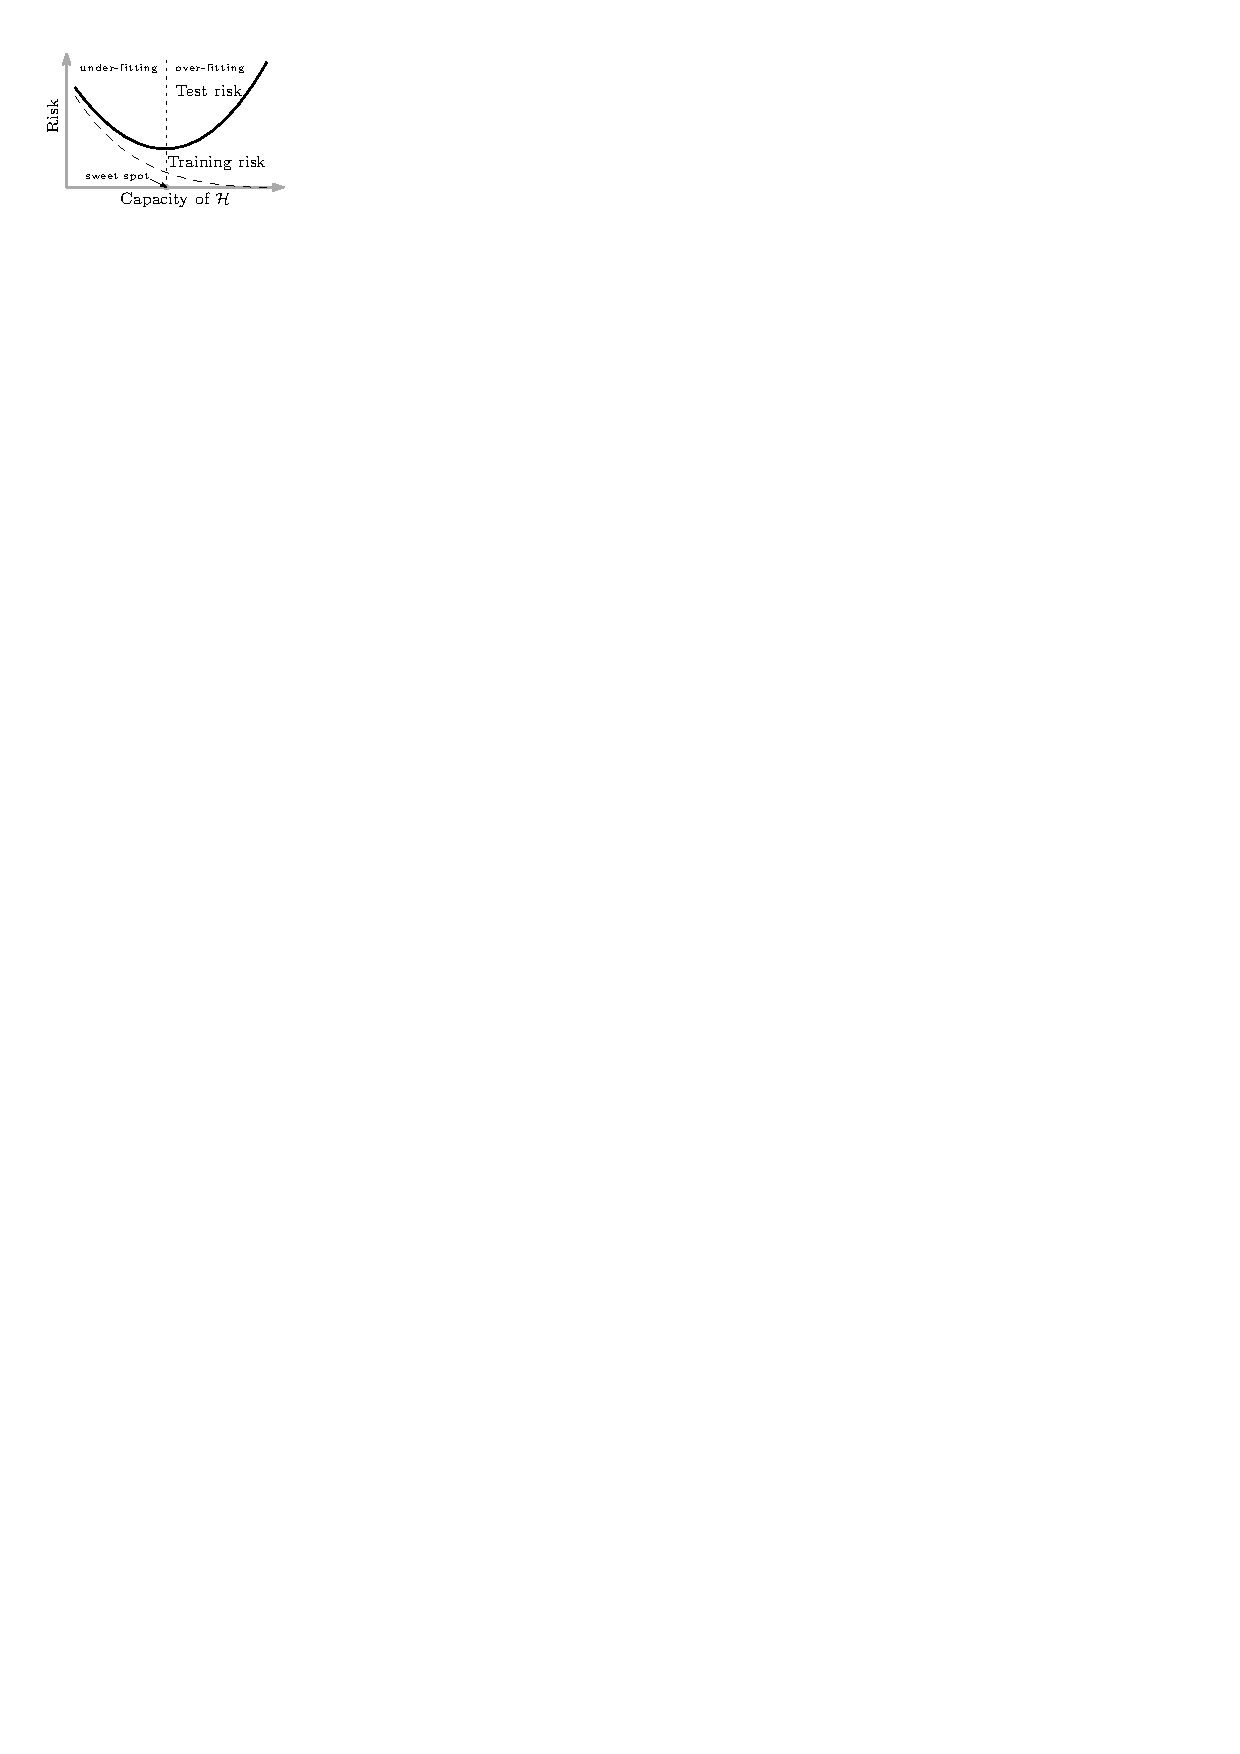
\includegraphics[height=0.13\textheight]{pdf/u-shaped.pdf} &
    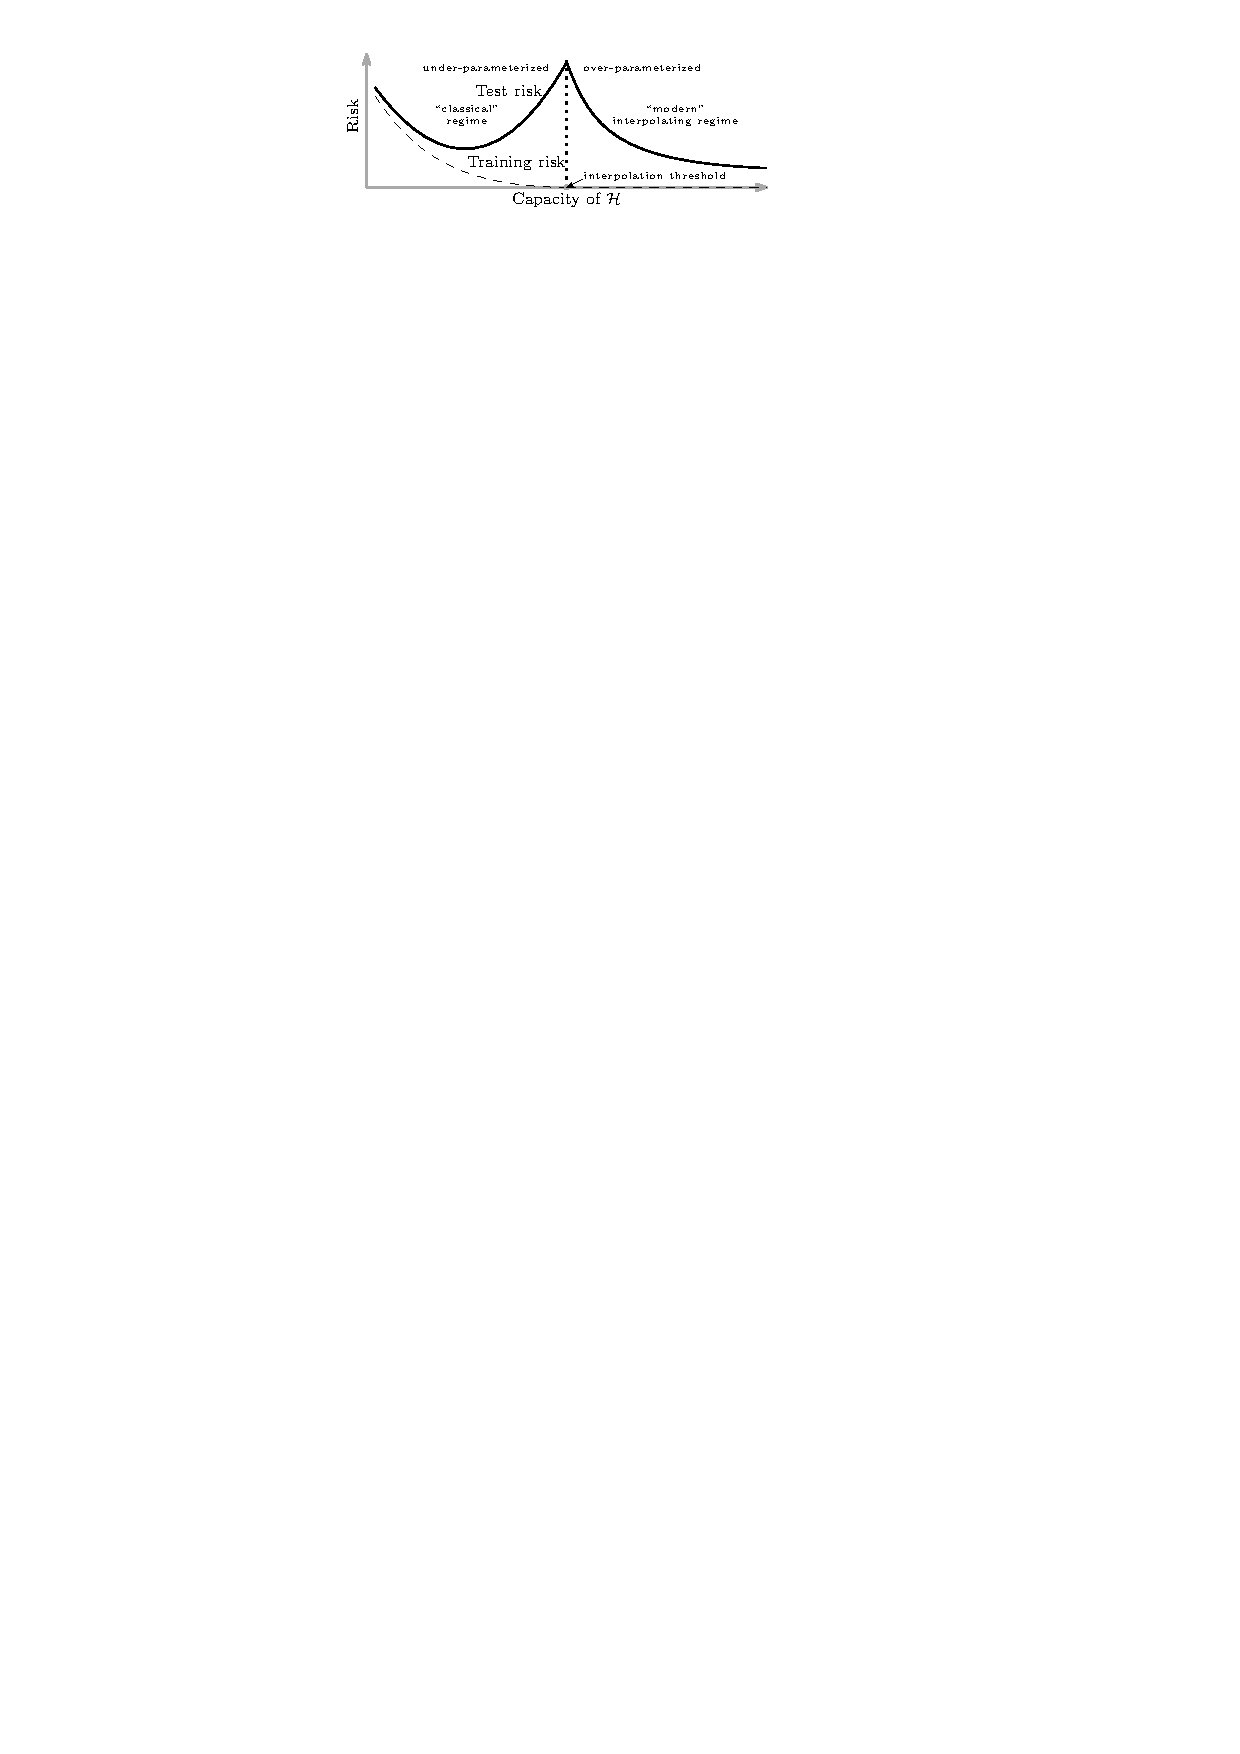
\includegraphics[height=0.13\textheight]{pdf/doubledescent.pdf} \\
    {\bf (a)} & {\bf (b)}
    \end{tabular}
    \caption{{\small {\bf Curves for training risk (dashed line) and test risk (solid line).}
      ({\bf a}) The classical \emph{U-shaped risk curve} arising from the bias-variance trade-off.
      ({\bf b}) The \emph{double descent risk curve}, which incorporates the U-shaped risk curve (i.e., the ``classical'' regime) together with the observed behaviour from using high capacity function classes (i.e., the ``modern'' interpolating regime), separated by the interpolation threshold.
      The predictors to the right of the interpolation threshold have zero training risk. Reproduced from \cite{belkin_reconciling_2019}.}}
    \label{fig:double-descent}
\end{figure*}

The main finding that Belkin found is a pattern for how the apparent performance on unseen data depends on model capacity and the mechanism underlying the emergence of double descent. When function class capacity is below the "interpolation threshold", learned predictors exhibit the classical $U$-shaped curve from Figure~\ref{fig:double-descent}. The `modern' interpolating regime marks the opposite trend to the right, where the risk starts to decrease up to a lower bound, which then can be called the \textit{optimal descent bound}. 

\blockquote[\cite{belkin_reconciling_2019}]{The bottom of the $U$ is achieved at the sweet spot which balances the fit to the training data and the susceptibility to over-fitting:
to the left of the sweet spot, predictors are under-fit, and immediately to the right, predictors are over-fit.
When we increase the function class capacity high enough (e.g., by increasing the number of features or the size of the neural network architecture), the learned predictors achieve (near) perfect fits to the training data---i.e., interpolation.
Although the learned predictors obtained at the interpolation threshold typically have high risk, we show that increasing the function class capacity beyond this point leads to decreasing risk, typically going below the risk achieved at the sweet spot in the ``classical'' regime.}

At this point, we would like to also clarify the term interpolation threshold in this case. Usually, under the pretext of overfitting and underfitting, interpolation threshold means the following: 

\begin{definition}[Interpolation threshold]
    Assuming a typical supervised learning setting, for a hypothesis $h$ within class structure $\mathcal{H}$, and a supposed concept $c$ of the class $\mathcal{C}$. Suppose $[X,Y]\subset c\in \mathcal{C}$ being the dataset, or \textit{observable space} of $c$ on which $h$ is tested on. Under the \textbf{empirical generalization learning} procedure, partitioning $[X,Y]$ into $[X,Y]_{1}$ and $[X,Y]_{2}$, for error evaluated on the first set, $\hat{R}_{1}(h)$ called training error, and the second set, $\hat{R}_{2}(h)$ called test error, with optimization applied on the first set, then evaluated statically on the second, the \textbf{interpolation threshold} with respect to a particular complexity measure of $h$, $\mathcal{M}(h)$, is the point $\mathcal{M}_{0}(h)$ where it is possible for $\hat{R}_{2}(h)/\hat{R}_{1}(h)\approx 1$, for $\hat{R}_{1}(h)\ll \epsilon$, $\hat{R}_{2}(h)\ll \epsilon$, with $\epsilon \geq 0$. 
\end{definition}

This basically means that what is learnt, with respect to the model complexity that gauge \textit{how much} and \textit{what} the model can learn, perfectly fits the concept $c$ itself, from the observation space on its own. We can say that, that specific sense, we gain the assumption that the observation space is \textit{fully representative} of the concept class, and the concept class is then fully realized by the model. Such point where that is possible, or there then such behaviour is possible, is called the interpolation point. The definition relies on the statement `where it is possible', hence it still, does not give us a particularly sound notion on to how and what constitute such possibility. The term empirical generalization learning comes from the fact that the procedure in practice of estimating and optimizing train-test-validation set in itself, is an imperfect empirical approximation of generalization testing. While the fact that we cannot gauge generalization error, in a purely blind black-box setting is settled (\cite{10.5555/2371238,10.5555/2930837,10.5555/2621980}), the method is then to try to mimic such by using generalization-via-hidden observations. To facilitate this, deliberately, the empirical learning procedure is only dynamic during training session, and static throughout the whole testing and validation testing section, and further on. 

By default, in general theory, such interpolating point is dangerous. Not only because it is inherently difficult to know exactly what the dataset constitute, whether it is actually representative of the concept that gives rise to it, or the structural information, noises, and interferences in between. It is hence impossible, to a certain point, to truly know the effectiveness of the model beside interpolating the current dataset which forms the observable details. 

Another prominent discovery to look at is \cite{nakkiran_deep_2019}, on the double descent of deep learning models. The paper serves as the first observation upon which double descent is observed on modern, deep learning theoretic models, especially complex one like Transformer or ResNet networks. 

\begin{figure}[htb]
    \centering
    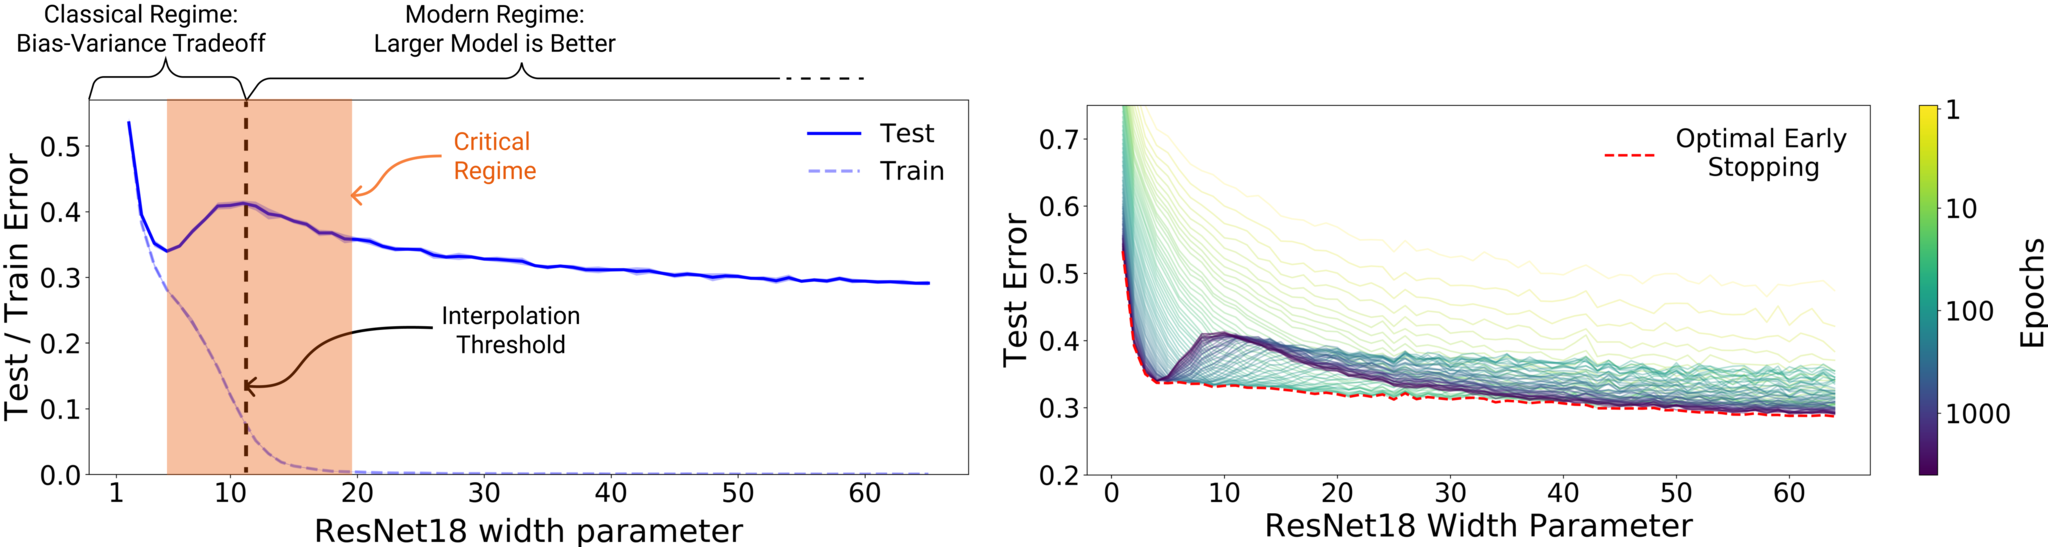
\includegraphics[width=\textwidth]{media/errorvscomplexity.png}
    \caption{{\bf Left:} Train and test error as a function of model size,
    for ResNet18s of varying width 
    on CIFAR-10 with 15\% label noise.
    %In the under-parameterized regime, test error follows
    %the behavior predicted by classical statistical learning theory, but in the overparameterized regime (once training error is approximately zero),  the test error undergoes a ``second descent'' and decreases as model size increases. The shaded region represents the critically parameterized regime where the transition from under- to over-parameterization occurs. 
    {\bf Right:}
    Test error, shown for varying train epochs.
    %The dashed red line shows that with optimal early stopping double descent is not observed.
    % All models are ResNet18s of varying width,
    % trained on CIFAR10 with 15\% label noise
    All models trained using Adam for 4K epochs.
    %, and plotting means and standard-deviations from 5 trials with random network initialization.
    The largest model (width $64$) corresponds to standard ResNet18. Resued from \cite{nakkiran_deep_2019}.
    %    \ptodo{point out that interpolation point for second plot is plotted in the ocean plot}
    }
    \label{fig:errorvscomplexity}
\end{figure}

\begin{figure}[htb]
\centering
\begin{minipage}{.512\textwidth}
  \centering
  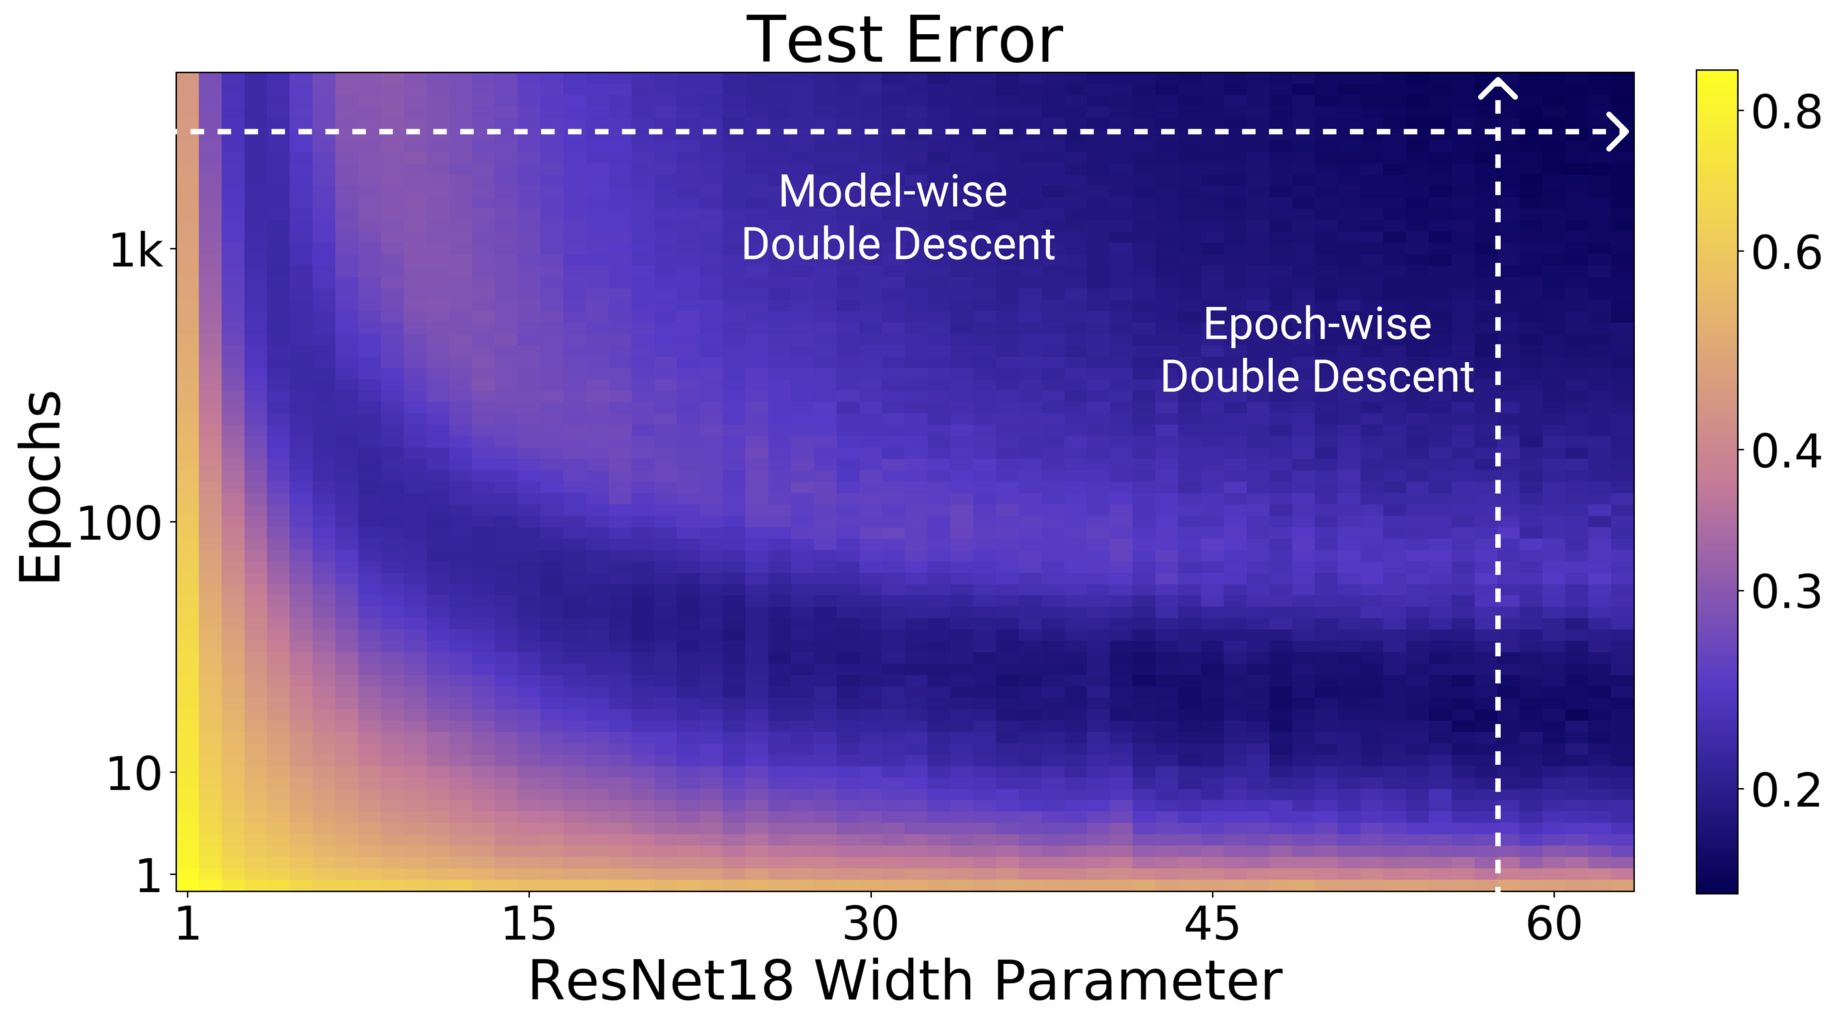
\includegraphics[width=1\textwidth]{media/introroc1.png}
\end{minipage}%
\begin{minipage}{.488\textwidth}
  \centering
  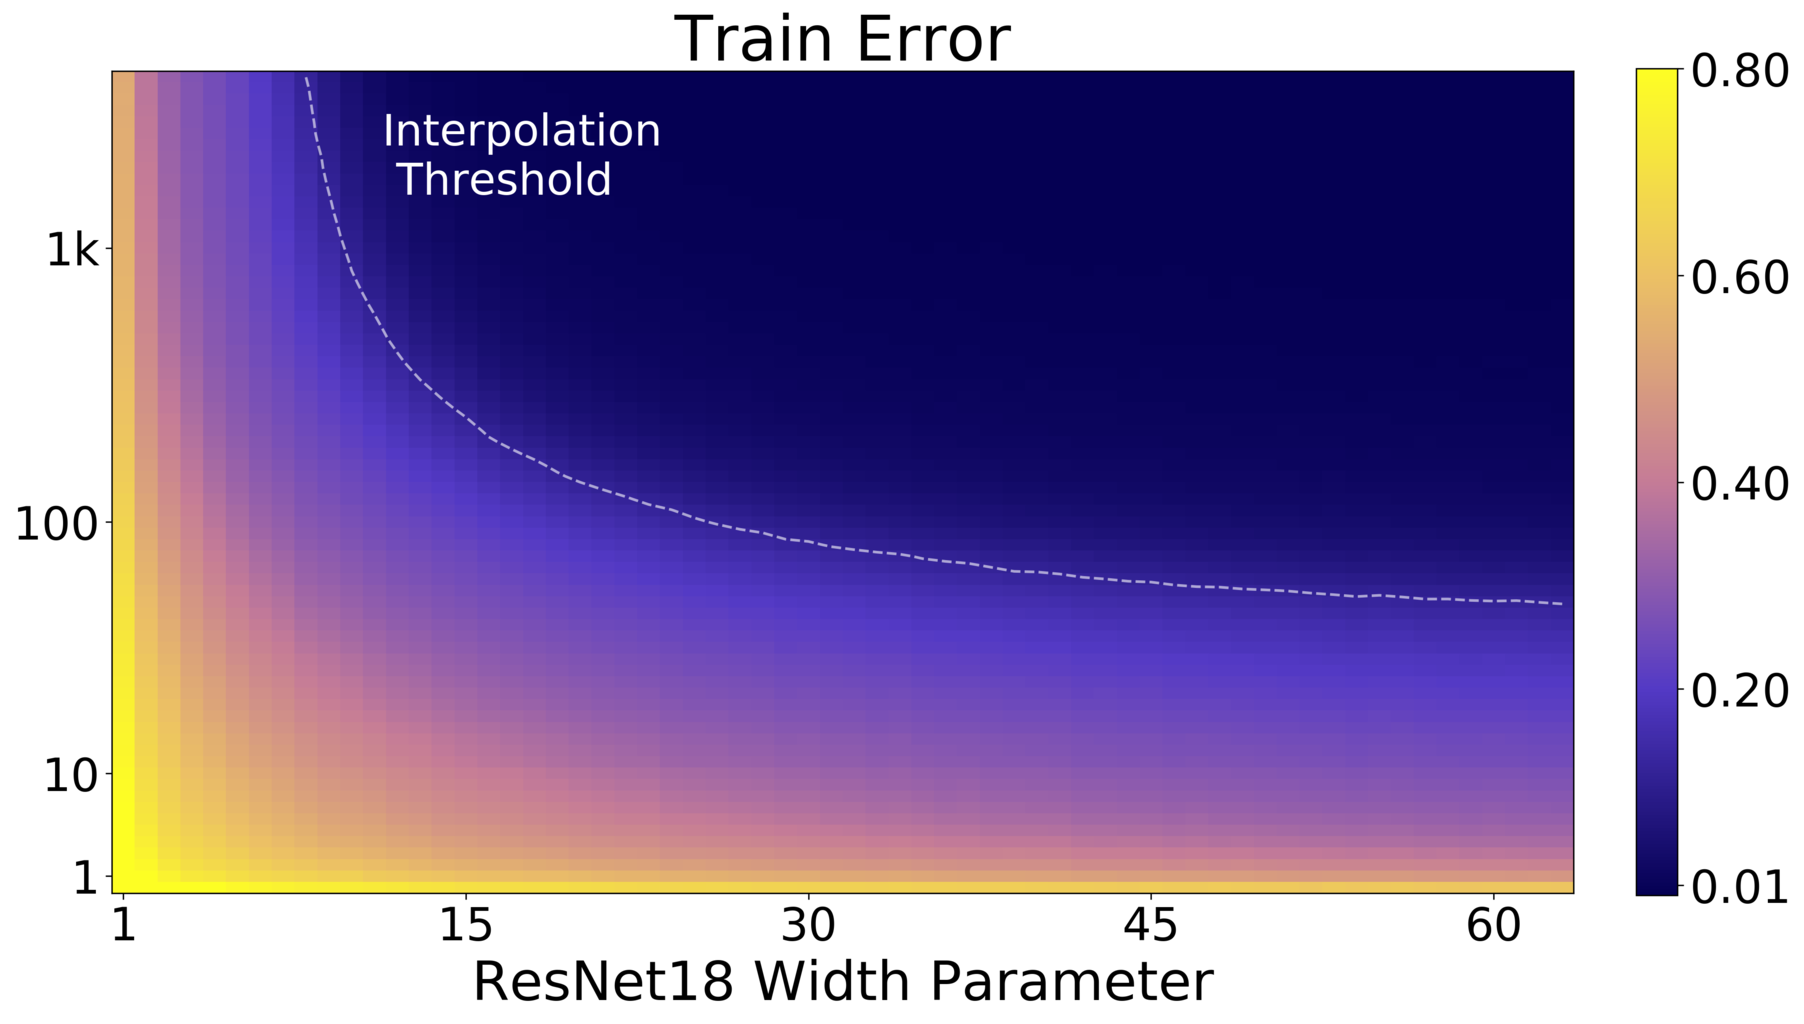
\includegraphics[width=1\textwidth]{media/introroc2.png}
\end{minipage}
\caption{{\bf Left:} Test error as a function of model size and train epochs. The horizontal line corresponds to model-wise double descent--varying model size while training for as long as possible. The vertical line corresponds to epoch-wise double descent, with test error undergoing double-descent as train time increases. {\bf Right} Train error of the corresponding models. All models are Resnet18s trained on CIFAR-10 with 15\% label noise, data-augmentation, and Adam for up to 4K epochs. Reused from \cite{nakkiran_deep_2019}}
\label{fig:unified}
\end{figure}

They define \emph{effective model complexity} of $\mathcal{T}$ (w.r.t. distribution $\mathcal D$) to be the maximum number of samples $n$ on which $\mathcal{T}$ achieves on average $\approx 0$ \emph{training error}. This is an entirely empirical definition, similarly per definition as VC-dimension. 

\newcommand{\EMC}{\mathrm{EMC}}
\begin{definition}[Effective Model Complexity]
The \emph{Effective Model Complexity} (EMC) of a training procedure $\cT$, with respect to distribution $\cD$ and parameter $\epsilon>0$,
is defined as:
\begin{align*}
    \EMC_{\cD,\eps}(\cT)
    :=  \max \left\{n ~|~ \E_{S \sim \cD^n}[ \mathrm{Error}_S( \cT( S )  ) ] \leq \eps \right\}
    \end{align*}
    where $\mathrm{Error}_S(M)$ is the mean error of model $M$ on train samples $S$.
\end{definition}

Using this definition, their main hypothesis can then be stated as the following three-fold regions:

\begin{hypothesis}[Generalized Double Descent hypothesis, informal] \label{hyp:informaldd}
For any natural data distribution $\cD$, neural-network-based training procedure $\cT$, and small $\epsilon>0$,
if we consider the task of predicting labels based on  $n$ samples from $\cD$ then:
\begin{description}
    \item[Under-parameterized regime.]  If~$\EMC_{\cD,\epsilon}(\cT)$ is sufficiently smaller than $n$, any perturbation of $\cT$ that increases its effective complexity will decrease the test error.
    \item[Over-parameterized regime.] If $\EMC_{\cD,\epsilon}(\cT)$ is sufficiently larger than $n$,
    any perturbation of $\cT$ that increases its effective complexity will decrease the test error.
    
    \item[Critically parameterized regime.] If $\EMC_{\cD,\epsilon}(\cT) \approx n$, then
    a perturbation of $\cT$ that increases its effective complexity
    might decrease {\bf or increase} the test error.
\end{description}
\end{hypothesis}

It is to notice that this definition is also only observational. By that, it only outlines the specific region of interest where the paradigm shift is identified through experimental results. It has no effective predictive power, or rather descriptive power more than setting up hypothesis with respect to the effective model complexity, and some arbitrary perturbation. \cite{nakkiran_deep_2019} also noticed this difficulty in providing a theoretical definition and theorem regarding such hypothesis, as said in their manuscript. The existence of the critical regime is also not defined. 

The behaviour itself has been particularly investigated, in certain settings. For example, before \cite{belkin_reconciling_2019}, \cite{advani2017highdimensionaldynamicsgeneralizationerror} investigated the generalization error in neural networks of high-dimensional measure. Of such, various behaviours that bear similarity to double descent can be observed. \cite{belkin2018understanddeeplearningneed} expanded on his previous research on the particular subset of kernel learning models, providing a theoretical analysis of specifically the Laplacian kernel on standard neural network. \cite{mei2020generalizationerrorrandomfeatures} investigated random feature regression in such regard, and also found similar results. 

The fact that double descent is not well-defined itself is a problem on its own. Up to the author's knowledge and of myself, there has been no effective definition or given description that outlines specifically how double descent can be structured. Instability in reproducing experiments and the effective range of the phenomena remains a question on its own. 

\noindent\rule{\textwidth}{0.4pt}


Ever since \cite{belkin_reconciling_2019}, despite the general chaotic view of double descent that seems to hold up pretty well, many researches have been conducted throughout, trying to observe or explain it, as we briefly mentioned \cite{nakkiran_deep_2019} as one of such main paper. Before attempting to do anything, and to further contribute with hypotheses forward, we will have to resolve to review previous coursework on such matter. Most of those works include some on theoretical analysis, some on dissection of optimization method then speculation of possible hindsight, some on experiments and observable effects, and so on. Furthermore, sections specifically designed to host experiments and observations will also offer a clearer insight into how this can be done. 

\noindent\rule{\textwidth}{0.4pt}

\section{Current researches}

The main goal of attacking double descent stemmed from the observation in which there exists irregularity in the model expression behaviours. As such, the first thing to do is to contrive the consensus on `what' constitutes double descent, at least per observable results, by delivering a conjecture. We deliver the phenomenological conjecture as below. 

\begin{conjecture}
    On the landscape of double descent, model complexity versus generalization error, there exists a fundamental point $\mathcal{M}_{0}$ of model complexity axis, where $dR(h)/d\mathcal{M}< 0$ for $\mathcal{M}> \mathcal{M}_{0}$, which is the interpolation point. 
\end{conjecture}

While this is not perfect, it provides us with a general idea on where to look for double descent. Typically, question remains as to see: 

\begin{enumerate}
    \item What is exactly double descent? As far as we can say, there exists the interpolation threshold in which the dynamic changes, but don't know why. Such exists and occur within the complexity of deep neural networks, and so is also analogous form in classical models. It is suspected, reasonably so, that it is related to the terms of bias-variance, however, it is not fully developed and no further inquiry is made beside the above conjecture as empirical observations. 
    \item Where does it lead? What is the setup? In truth, the setup problem in machine learning has been quite troubling. As mentioned, statistical theory lives in the idealized system, and thus many of its bounds hold in such domain. However, there exists the fundamental mismatch between how models are in practice, or rather in a semi-theoretical regime, compared to the rigidity of classical systems. The setup itself is then impractical, for example of the assumption in which the distribution drew out of $x$ is fully Gaussian, or isotropically Gaussian, which is not helpful in practice. 
    \item What counts as the measure, and what we even measure? This is more of the concern toward what counts as model complexity, and the structural constraints that comes with it. Usually this is directed toward neural network, but even then, parameter-based complexity is often a poor choice of representation, thus begs the question what is even it, and why suddenly it appears there, within the dynamic of such?
    \item Why would such an optimization space induce double descent? Surpassing what we have, the bounds that we are having indicates the strong trajectory in which downward trend is the only way, as for the generalization capacity is increased by increased transparency, i.e. $|\mathcal{S}|$ of the observation set, and by increased capacity $|\mathcal{H}|$ on certain induced or `natural system' (convex system topology). However, this seems to not be the case. 
\end{enumerate}

With this, we are ready to follow up the literatures in provision of said questions. Let us also recite what happens within the setting of many double descent results. 

\subsection{Discovery of double descent}
While double descent is discovered by \cite{belkin_reconciling_2019} and further on modern deep learning landscape of \cite{nakkiran_deep_2019}, it remains that the conclusion is not reached if there exists some fundamental models that would not have double descent, the consistency of double descent through different models entirely and so on. This is mainly because of a particular `shock effect', since before double descent, bias-variance holds the candle as the main principle of choosing and optimizing models to its optimal saddle point. Suddenly by then we observe double descent, which introduces the interpolating threshold $\mathcal{M}_{0}$, that breaks this principle. There is then the open question on how far-reached is double descent in consideration of different architectures, and this is reflected in several papers above. As of now, the main structures that have been verified includes
\begin{itemize}[topsep=1pt, itemsep=1pt]
    \item \textbf{Classical models} \cite{Yang_2024,nakkiran2019moredata,schaeffer_double_2023,lafon_understanding_2024} (linear regression and classical polynomial), \cite{NEURIPS2024_2d43f7a6} (linear regression upon least square), \cite{liu2021kernelregressionhighdimensions}, \cite{zhang2024manipulatingsparsedoubledescent,allerbo2025changingkerneltrainingleads} (kernel methods/regressions), \cite{brellmann2024on} (Classical MSBE-LSTD\footnote{Mean-Squared Bellman Error and Least-Squared Temporal Difference} optimization), \cite{harzli2023doubledescentcurvesneuralnetworks} (Gaussian process). Some papers also have experiments on Random Fourier Feature Networks, and so on, but not substantial (including \cite{belkin_reconciling_2019} paper). 
    \item \textbf{Deep neural networks}: \cite{luo2023doubledescentdiscrepancytask,Yang_2024,pezeshki2021multiscalefeaturelearningdynamics} (CNN, VGG, ResNet, and DenseNet), \cite{nakkiran_deep_2019} (Transformer), \cite{shi2024homophilymodulatesdoubledescent} (GNN). 
\end{itemize}

Most of the experiments are concerned of seeing and analysing double descent, basic analysis and experimental observations, test case scenarios for different models and setting and so on. All of the above models are then considered to be, concretely, reported of observing double descent, through various testing scenario on them. Review papers and literatures can be found as \cite{schaeffer_double_2023,ErdongHu2021}, and \cite{shi2024homophilymodulatesdoubledescent} on specifically, graph neural network. However, GNN would requires its separated discussion, so we will only briefly mention it as such. 

\subsection{Theoretical attacks}

Because of its intrinsic nature, where double descent breaks the long-standing principle of learning selection, theoretical resolutions has been employed to tackle such problem. Indeed, for example, \cite{cherkassky2024understand} and \cite{lee2022vctheoreticalexplanationdouble} aim toward such direction by understanding the behaviours of double descent using the classical VC-theory approach. However, such papers only introduce, or relate double descent to VC-theory via phenomenological approach - for example, reducing the VC-dimension while fixing or reducing training error, or by examining a potential proxy between the VC-bounds and potential factors encapsulated in the quantities involved. They however, do raise voices of certain inherent problems lies within the theory of learning and in general, learning models. 

Beyond such, certain discovery and inquiries help in having a clearer picture on the behaviour of double descent through various structures. For example, \cite{hastie2019surprises}, under pretext of studying high-dimensional ridgeless ($\ell_{2}$ norm) interpolation, analyse the case of \textit{isotropic features}, \textit{correlated features}, misspecified model (feature observation inhibited), on ridgeless interpolation of linear model, and soon as nonlinear model and latent space model. While strong, their results are restricted to a specific class of assumptions and structure, and is doubtful to be extended further. \cite{allerbo2025changingkerneltrainingleads} investigated and find a particular double descent trace when changing kernel during training, specified in the term of the minimum allowed bandwidth. The kernel bandwidth $\sigma\geq 0$ of a specific kernel filter determines the information smoothing, hence implies the complexity abides by the kernel structure, as well as determine the smoothness of information indicted by the term. 

The sentiments that are shared in between researchers on the topic of double descent vary, but have some common roots, most of them coming from the difficulty to fully assess double descent and its factor components. While double descent concerns the evaluation of \textit{generalization (test) error}, and the \textit{model complexity} notions, the error in question is often implicitly defined or loosely considered in one way or another, and model complexity has no consensus on its definition. In fact, this points out a very potential, if not already mismatch in the theoretical development. While optimizations and phenomenological aberration of models, as well as building and constructing models at will are well-developed, the definitions on which they are defined on is not fully understood, if not undefined. As of now, literatures on model complexities like \cite{modelcomplex_exp,hu_model_2021,janik2021complexitydeepneuralnetworks,truong2025rademachercomplexitybasedgeneralizationbounds,luo2024investigatingimpactmodelcomplexity} introduce their variations or a copula of different definitions altogether, where some are concerned with its effective complexity, some are concerned with its expressive or structural complexity with different ways to define the model underneath, from parameters to units, to random standard variables (\cite{neal2018modern}). There is also the rift in consideration between classical theory, of which mainly is for classical models, and modern deep neural network structures of which do not conform to such analysis.

\subsection{High-dimensional ridgeless interpolation - \cite{hastie2019surprises}}
Aligning with our previous experiments, \cite{hastie2019surprises} conducted investigation into the class of ridgeless approximation criterion on linear-nonlinear classes disparity. The investigation itself is thorough in parameter-term. Specifically, they investigated the case of which we have \textbf{isotropic features}, where asymptotic risk depends on the weight $w$ only through its norm $||w||_{2}$; \textbf{anisotropic features}, where the model risk depends on the geometry of the pair $(\Sigma, w)$ for $\Sigma = \mathrm{Cov}(x_{i})$ on the dataset $(y_{i},x_{i})^{n}_{i\leq n}\in\mathcal{S}$; and the case of nonlinear model, where the model itself is tested with added structure - $x_{i}$ is obtained by passing $z_{i}\sim\mathcal{N}(0,I_d)$ through a one-layer neural network with random first layer weights.  

Overall, the research itself is rather insightful, 

\subsection{Sample-wise double descent - \cite{nakkiran2019moredata}}

Regarding double descent, \cite{nakkiran2019moredata} explored the problem, in which the increment of sample actually hurts linear regression process. As always, the setting considers isotropic $x\sim\mathcal{N}(0,I_{d})$. Here, the observation and claim is that the number of samples can indeed, hurt the end result for test MSE on the model. This results intwo two claims, mainly of the decomposing bias-variance analysis. First is the overparameterized risk claim, in which is defined of:

\begin{claim}[Overparameterized Risk]
\label{claim:main}
Let $\gamma := \frac{n}{d} < 1$ be the underparameterization ratio.
The bias and variance are:
\begin{align}
B_n &= (1-\gamma)^2||\beta||^2\\
V_n &\approx \gamma(1-\gamma)||\beta||^2
+ \sigma^2 \frac{\gamma}{1-\gamma}
\end{align}
And thus the expected excess risk for $\gamma < 1$ is:
\begin{align}
\E[\bar R (\hbeta) ]
&\approx (1-\gamma)||\beta||^2
+ \sigma^2 \frac{\gamma}{1-\gamma}\\
&= (1-\frac{n}{d})||\beta||^2
+ \sigma^2 \frac{n}{d-n}
\end{align}
\end{claim}
and the second one is about the underparamterized case, which is as the second claim. 
\begin{claim}[Underparameterized Risk, \cite{hastie2019surprises}]
\label{claim:underparam}
Let $\gamma := \frac{n}{d} > 1$ be the underparameterization ratio.
The bias and variance are:
\begin{align*}
B_n = 0 \quad, \quad
V_n \approx \frac{\sigma^2}{\gamma - 1}
\end{align*}
\end{claim}

Those claims are troublesome, in the sense that they indict heavily on the assumptions of which, for example, suddenly the bias collapse to zero without any indication or further justification. The variance is specifically designed for a replica-style curve fitting instead, of which the approximating relation suggest the not-so-useful notion, in which such deviation from the claim can be wide and far yet still right in terms of descriptive behaviours (converges to $0$). Vanishing terms transition from the first claim to the second claim inherently accept bias of the system itself, of which is then trouble some to proceed against. And the list of assumptions on fine structures are too many in spirit, especially the linear algebra mapping in which derivations of computation are used in the paper itself. To truly justify this, we need something beyond what is described here. 

\subsection{Multiscale feature learning dynamics - \cite{pezeshki2021multiscalefeaturelearningdynamics}}


\subsection{Reinforcement learning and double descent - \cite{brellmann2024on}}


\subsection{Out-of-Distribution Detection - \cite{ammar2025doubledescentmeetsoutofdistribution}}


\subsection{Gaussian processes and neural network - \cite{harzli2023doubledescentcurvesneuralnetworks}}


\subsection{Double descent on GNN - \cite{shi2024homophilymodulatesdoubledescent}}


\subsection{Weak feature double descent - \cite{Belkin_2020}}


\subsection{Grokking, Emergence, and Double Descent - ~\cite{huang2025samplecomplexityrepresentationability}}

\subsection{Variations on analysis}
Many sub-variations and analysis alongside major substantiated discoveries listed above can help in analysis. Some of them are toward linking different existing dynamics to large neural network in non-linear fashion, or generalizing approximation of linear network toward nonlinear systems. 
\subsubsection{Dropout and double descent - \cite{Yang_2024}}

Dropout is a relatively well-established regularization technique for training deep neural networks, usually by exclusion of different neurons during processes, as seen i \cite{srivastava2014dropout} to control overfitting. Accordingly, \cite{Yang_2024} predicted or stated that regularization techniques can nullify double descent, and thus also dropout. The model considered is linear regression model, for $p$ covariates $x\in\mathbb{R}^{p}$ and response or output $y\in\mathbb{R}$ are related by \begin{equation}
    y = x^{\top}\beta_{0}+\epsilon , \quad \epsilon \sim \mathcal{N}(0,\sigma^{2})
\end{equation}
The situated dropout is as followed. Given training data $z^{n}=\{(x_{i},y_{i})\}^{n}_{i=1}$, for $X=[x_1,\dots,x_n]^{\top}$ and $y=[y_{1},\dots,y_{n}]^{\top}$, the estimation of weight $\beta$ by $\hat{\beta}(z^n)$ (model's weight), to minimizing the training error 
\begin{equation}
    \underset{r\sim\mathcal{B}er}{\mathbb{E}} || y - (r\odot X)\beta ||^{2}_{2} = ||y-\gamma X\beta||^{2}_{2} + (1-\gamma)\gamma ||\Gamma \beta ||_{2}^{2}
\end{equation}
for $\odot$ denoting the element-wise product on $L^{2}$ norm space, each element of $R\in\mathbb{R}^{n\times p}$ takes one and zero with probabilities $\gamma$ and $1-\gamma$, for the distribution $\mathcal{B}er(\gamma)$ corresponding to such, and $\Gamma = \diag{(X^{\top}X)^{1/2}}$. The final description gives the form of the effective dropout objective. Originally from the paper, they consider it exactly of a Tikhonov regularization method. Set $\beta'=\gamma \beta$, then \begin{equation}
    \begin{split}
        &||y-X\beta'||_{2}^{2} + \frac{1-\gamma}{\gamma} ||\Gamma \beta'||^2, \\
        &\hat{\beta}_{n\gamma} = \left(X^{\top}X+\frac{1-\gamma}{\gamma}\Gamma^{\top}\Gamma\right)^{-1}X^{\top}y
    \end{split}
\end{equation}
minimization. While experiments regarding such regularization works in such domain and was illustrated as to be reasonably effective, fallacies in claims and insight remains, especially in the nullification of double descent. The problem here is that, any given amount of dropout is, accordingly to the author, similar to Tikhonov or ridge regularization on structural complexity. As explained in the $c'$ optimization of $c$-space in preliminary sections, such induces a different, much smaller system in which the additional structural attractor points toward the region of low regularizing complexity throughout the domain. Such superposition between the $\{\lambda r(h)\}(\mathbb{R})$ landscape and the classical loss $\hat{R}$ only morph the dynamic setting to a different region, and thereby bypass double descent in such case for absolute non-overfitting convergence to $\min{(\hat{R}_{\mathcal{S}}(h))}$. This works well on well-behaved and loosely stable case, but in a lot of scenarios, such cannot be guaranteed, especially for pathological systems. Furthermore, Speaking in terms of the \textit{inductive bias}, mismatch between model and effective regularization becomes a problem, as there exists no effective complexity measure for the regularization term $r(h)$. Some are ill-conditioned, for example, $r(h)=\sum_{j}w_{ij}^{2}$ for square terms $ij$-indexed weights only take into account the reasonable weight system, without the semantic itself, or meaningful weights. A forced dropout might potentially in certain less ideal cases, be more destructive, and introduces double descent back again, until the stochastic process shifts meaningful weight to a more resource constrained system. This means we have to induce, or at least formalize if stochastic process can recover meaningful semantic after dropout randomly. We can test this somewhat, by introducing a small toy test on the proposed dropout estimator: 
\begin{theorem}[Expected test error, \cite{Yang_2024}]
    Let $\alpha = C< \frac{1}{(1+\sqrt{p/n})^2}$, the expected test error is \begin{equation}
        f(\alpha) = \left\{ 1- a\alpha + 2\alpha^2 \frac{p}{n} \right\} ||\beta_{0}||^2 + \sigma^2 \alpha^2 (\alpha + 1)\frac{p}{n} + O\left(\frac{1}{n^2}\right)
    \end{equation}
    with $\alpha=\gamma/(1-\gamma)$.
\end{theorem}
While the theorem is proved, we then must know if such theorem correctly correlates to even small dynamic systems.

\section{Problems}
There are a lot of problems regarding how we treat the problem, how we see it, and how we actively analyze it. Most of them lies in the space of statistical learning theory, since bias-variance on itself has variations and justification that is seemingly very natural in statistical theory, like the other version name \textit{approximation-estimation error tradeoff}. All of them contribute somewhat to the current outlook, and so far, it has been pretty bad, than what is being advocated of. Nevertheless, let us state them out, even if missing some particular details. 

\subsubsection*{Problem 1. Authoritative statements}
Despite its prevalence in particular research interest, double descent itself has no definite statement to describe its particular behaviour. This is also true for a list of other phenomena, such as \textit{grokking} (\cite{power2022grokkinggeneralizationoverfittingsmall}), \textit{emergence behaviours} (\cite{wei2022emergentabilitieslargelanguage}, typically discussed in large language models, which is understandable of large-scale specific ruling system), \textit{implicit bias} (\cite{soudry2024implicitbiasgradientdescent}), and \textit{neural scaling law} (\cite{kaplan2020scalinglawsneurallanguage,wei2022emergentabilitieslargelanguage}). There is also \textit{catastrophic forgetting} (\cite{vandeven2024continuallearningcatastrophicforgetting}) which is still fairly native of large systems; nevertheless, those phenomena will be of target later on (or discussed in later chapters). The fact remains that we only \textit{partially understand} these particular results with conjectures and theories to support the facilitation of new insights, new analytical lens, and nothing much. Without a clear definition of what is even double descent, sometimes, we cannot proceed, lest to say even solving it. This is a problematic issue, since the current theory is so messy and not rigid that many even turns to exotic choices, like topological informatics learning theory, \textit{Homotopy Theoretic and Categorical Models} (\cite{Manin_2024}), and several more. Without clear definitions, it remains ambiguous whether double descent constitutes a single phenomenon, a family of related behaviours, or an artefact of particular modelling and evaluation choices. 

More fundamentally, the term \textbf{double descent} does not currently admit a formal definition beyond an empirical characterization of observed risk behaviour. While several works have suggested interpreting double descent as an instance of emergent behaviour, such interpretations necessarily remain conjectural, as emergence itself lacks a precise and operational definition within contemporary learning theory. As a result, appeals to emergence do not resolve the underlying indeterminacy of the phenomenon, but rather shift it to a different conceptual level.

Empirically, double descent has been reported in a variety of settings, while being absent in many others, even under closely related modelling and data conditions. This variability complicates attempts to treat double descent as a unified phenomenon and raises the question whether it constitutes a single mechanism, a collection of regime-dependent effects, or an artefact of specific modelling and evaluation choices. In the absence of necessary and sufficient conditions for its occurrence, theoretical accounts are forced to accommodate mutually incompatible behaviours, thereby undermining their explanatory specificity. Consequently, existing frameworks face a dual difficulty: they neither reconcile naturally with classical bias-variance analyses, nor align with the assumptions underlying earlier generalization results, such as uniform convergence over well-behaved hypothesis classes. Without a precise characterization of the object under study, it remains unclear how such theories can be systematically compared, falsified, or extended.

\subsubsection*{Problem 2. Model complexity}
The notion of model complexity has undergone a significant conceptual shift in the recent literature. Several works have attempted to formalise or reinterpret model complexity in modern learning systems \cite{hu2021modelcomplexitydeeplearning,luo2024investigatingimpactmodelcomplexity,barcelo2020modelinterpretabilitylenscomputational,Molnar_2020,janik2021complexitydeepneuralnetworks}. This problem becomes apparent when the inherently complex nature of contemporary models—particularly deep learning models based on multilayer perceptron (MLP) architectures—is examined, as such models cannot be treated analogously to classical hypothesis classes.

In \cite{hu2021modelcomplexitydeeplearning}, deep learning models are analysed through notions such as expressive capacity, effective capacity, VC dimension, and proxy-based Rademacher complexity bounds, alongside perspectives grounded in functional analysis, computational complexity, and representational width. However, these approaches remain largely heterogeneous and regime-dependent. Notably, \cite{Molnar_2020} demonstrates the possibility of decomposing model behaviour into multiple contributing notions of complexity, suggesting a unification at the level of functional variation rather than a single scalar measure.

Despite these advances, there remains no conclusive or universally accepted definition of model complexity. This ambiguity becomes particularly problematic in light of phenomena such as double descent, which have been observed not only in deep learning models but also, inconsistently, in classical settings \cite{belkin_reconciling_2019}. As a result, the issue is foundational: theoretical analysis of generalisation behaviour presupposes a well-defined notion of complexity, especially when complexity itself is the variable of interest.

Relatedly, the concepts of overparameterization and underparameterization lack precise and agreed-upon definitions. Their usage is often context-dependent and implicit, yet they play a central role in the classification of problem settings and the interpretation of learning dynamics. Without explicit characterisation of these notions, theoretical comparisons across models and regimes remain inherently ambiguous. Absent such definitions, claims relating model complexity to generalisation behaviour risk being descriptive rather than explanatory.

\subsubsection*{Problem 3. Model structure}

In modern practice, the theoretical and formal treatment, rigorous consideration of different model structures and complexity is not realized. Partially, this is due to the bloom of machine learning and artificial intelligence from the early 2000s. Currently, there has been no conclusive theoretical definition or formulation about the structure of different models, typically can go under the name of mathematical modelling hypothesis, in a way that unify certain properties between architectures. Heuristics are also often employed in several newer models and widely-utilized structures typically seen in large-scale systems, leading to difficulty in formalization and factorization of affectants. 

\subsubsection*{Problem 4. Theoretical insufficiency}

The setting surrounding the learning theory, machine learning models is generally missing of its rigours and analytical properties. Most of the learning setting and model's training-testing setting are often narrowly stated in theoretical sense, and there are a lot of diffusing details that might or might not affect the model's perturbation without knowing. This in a certain way leads to the complexity in analysing different problem setting and experimental results, since the architecture used, the setting considered, model in questions, configuration (either custom or on system side) are not consistent overall. 

Furthermore, a lot of terms, definitions are often hand-waived in papers or in discussions. This also led to the point that in \cite{nakkiran_deep_2019}, they have to somehow 'reinvent' another type of model complexity itself, albeit unsatisfying of a definition, is still a new kind of definition per insufficiently of such. while it is welcome to introduce new definitions, the fact is that it is subjectively inconclusive of terms, definitions and thereof leads to the perception and situation where multiple studies can be found, but all of them are defined on different ground.

Analysing statistical learning theory and overall landscape of statistical learning theory, and the learning theory as a whole, encountering new problems like double descent also revealed its weakness, and ultimately, perhaps one of the reason why it is ineffective against such problem. First, there are simply too many assumptions made, too many formulations made during said process. Furthermore, there are also unclear notions and concepts, of which make it even harder to analyse or fully formalize. Secondly, there are inherent conflicts and uncertainty within those theories, formulations and notions by itself. For example, in one sense, the No-free-lunch theorem is considered to be representative and true, whilst also simultaneously being considered the opposite of such. And amidst abnormality behaviours of the old bias-variance formulation, we also find distinctive weakness in our theory, for example, the concerning difficulty in defining the notion of \textit{model complexity} in various contextual ways. To analyse double descent, perhaps we also need a new theory or formulation to support it. \footnote{Furthermore, most of the general solution and bounds created by statistical learning theory is often in a very simplistic system. For example, if we are to utilize the Rademacher complexity measure (\cite{10.5555/2371238}), most of the time we will have to compute it through the growth function $\Pi_{\mathcal{H}}(m)$ for $m$ points, on the standard finite hypothesis class $\mathcal{H}$ such that 
\begin{equation}
    \Pi_{\mathcal{H}}(m) = \max_{x_1, \dots, x_m \in \mathcal{X}} \left| \left\{ (h(x_1), \dots, h(x_m)) \mid h \in \mathcal{H} \right\} \right|
\end{equation}
Most of our problems resolve to binary classification, or rather, the problem of pattern recognizing discrete, reduced classification form. It is not so sure for now if all problems can be reduced to such way, so we cannot draw conclusive analysis that is not diluted of mathematical formulation for complex systems. That is not to count the computationally intensive operation required to calculate the supposedly classical measure, while not entirely of itself holds any substantial reasonable information about the internal dynamics of the model itself. }

Another problem with classical analytical solution is that it is very \textit{loose}, almost too loose to even considered of such. But sometimes it is too \textit{rigid} in a sense such that it simply does not work at all. Indeed, basing our works and foundational assumptions on top of approximation theory is not quite good at all, because they are very limited. Overall, we can say it is not equipped for handling similar situation. For example, almost all bounds that is subjected of classical learning theory only guarantee particular existential theorem, under very simplified and specific situation without the virtue of extending it to a more general setting. 
